\documentclass[12pt,a4paper]{report}

\usepackage[T1]{fontenc}
\usepackage[utf8]{inputenc}
\usepackage[french]{babel}
\usepackage{geometry}
\usepackage{graphicx}
\usepackage{float}
\usepackage{array}
\usepackage{longtable}
\usepackage{booktabs}
\usepackage{hyperref}
\usepackage{xcolor}
\usepackage{enumitem}
\usepackage{fancyhdr}
\usepackage{titlesec}
\usepackage{tikz}
\usetikzlibrary{positioning,arrows.meta,calc,shapes.geometric}

\geometry{margin=2.5cm}
\setlength{\headheight}{15pt}
\setlist[itemize]{leftmargin=1.4em}
\setlist[enumerate]{leftmargin=1.6em}
\graphicspath{
  {../diagrams/uml_actuel/}
  {assets/organigrammes/}
  {maquettes/desktop/}
  {maquettes/desktop/admin/}
  {maquettes/desktop/client/}
  {maquettes/desktop/gestionnaire/}
  {maquettes/desktop/responsable/}
  {maquettes/desktop/archiviste/}
  {maquettes/desktop/auditeur/}
  {maquettes/rapport/desktop/}
  {assets/logos/}
  {assets/plantuml/}
}

\definecolor{sonacosgreen}{RGB}{24,86,55}
\definecolor{sonacosred}{RGB}{220,35,45}
\definecolor{softgray}{RGB}{245,247,245}

\tikzset{
  orgMain/.style={
    draw=sonacosgreen,
    very thick,
    rounded corners=4pt,
    fill=sonacosgreen!8,
    align=flush center,
    text width=4.4cm,
    minimum height=0.95cm,
    inner xsep=6pt,
    inner ysep=5pt,
    font=\bfseries,
    execute at begin node={\hyphenpenalty=10000\exhyphenpenalty=10000\relax}
  },
  orgBox/.style={
    draw=black!55,
    rounded corners=3pt,
    fill=white,
    align=flush center,
    text width=3.15cm,
    minimum height=0.88cm,
    inner xsep=5pt,
    inner ysep=4pt,
    font=\small,
    execute at begin node={\hyphenpenalty=10000\exhyphenpenalty=10000\relax}
  },
  orgService/.style={
    draw=black!45,
    rounded corners=3pt,
    fill=softgray,
    align=flush center,
    text width=2.85cm,
    minimum height=0.82cm,
    inner xsep=4pt,
    inner ysep=4pt,
    font=\footnotesize,
    execute at begin node={\hyphenpenalty=10000\exhyphenpenalty=10000\relax}
  },
  orgServiceWide/.style={
    orgService,
    text width=3.15cm
  },
  orgLine/.style={draw=black!60, line width=0.55pt}
}

\hypersetup{
  colorlinks=true,
  linkcolor=sonacosgreen,
  urlcolor=sonacosgreen,
  citecolor=sonacosgreen
}

\pagestyle{fancy}
\fancyhf{}
\lhead{\textcolor{sonacosgreen}{Plateforme web SONACOS}}
\rhead{\thepage}
\renewcommand{\headrulewidth}{0.4pt}

\titleformat{\chapter}
  {\normalfont\huge\bfseries\color{sonacosgreen}}
  {Chapitre \thechapter :}{0.6em}{}

\titleformat{\section}
  {\normalfont\Large\bfseries\color{sonacosgreen}}
  {\thesection}{0.6em}{}

\titleformat{\subsection}
  {\normalfont\large\bfseries}
  {\thesubsection}{0.6em}{}

\newcommand{\blankline}{\vspace{0.4cm}}
\newcommand{\desktopfigure}[3]{
\begin{figure}[H]
  \centering
  \fbox{\includegraphics[width=0.92\textwidth,height=0.48\textheight,keepaspectratio]{#1}}
  \caption{#2}
  \label{#3}
\end{figure}
}

\begin{document}
\pagenumbering{gobble}

\begin{titlepage}
  \centering
  \makebox[\textwidth][c]{
\includegraphics[width=1.12\textwidth,height=4.6cm,keepaspectratio]{emsi-honoris-logo-cropped.png}}

  \vspace*{1.2cm}
  {\Large \textbf{Rapport de Projet de Fin d'Année}}\par
  \vspace{0.5cm}
  {\large 4ème année -- Développement Digital et Systèmes d'Information}\par
  \vspace{1.5cm}

  {\large \textbf{Sous le thème}}\par
  \vspace{0.6cm}
  \rule{\textwidth}{0.6pt}\par
  \vspace{0.6cm}
  {\LARGE \textbf{\textcolor{sonacosgreen}{Conception et réalisation d'une plateforme web de gestion commerciale et e-commerce pour SONACOS}}}\par
  \vspace{0.6cm}
  \rule{\textwidth}{0.6pt}\par

  \vspace{1.5cm}
  {\Large \textbf{Application web SONACOS}}\par
  \vspace{0.3cm}
  {\large Semences, engrais, commandes, stock, paiements, factures et administration}\par

  \vfill

  \begin{minipage}{0.40\textwidth}
    \raggedright
    \textbf{Réalisé par :}\\
    Mohamed Amine Bensserrar
  \end{minipage}
  \hfill
  \begin{minipage}{0.50\textwidth}
    \raggedright
    \textbf{Encadré par :}\\
    Encadrant pédagogique :\\
    M. Elgerari Oussama\\[0.2cm]
    Encadrante de stage :\\
    Mme Meryem Setti
  \end{minipage}

  \vfill
  {\large Année universitaire : 2025--2026}\par
\end{titlepage}

\pagenumbering{roman}

\chapter*{Dédicaces}
\addcontentsline{toc}{chapter}{Dédicaces}

Je dedie ce travail a ma famille pour son soutien, sa patience et ses encouragements tout au long de mon parcours académique. Son accompagnement a constitue une source essentielle de motivation durant la réalisation de ce projet.

Je dedie egalement ce projet a mes enseignants et encadrants, qui ont contribue a ma formation et m'ont permis d'acquerir les compétences nécessaires pour mener une demarche complète d'analyse, de conception et de développement.

Enfin, je dedie cette réalisation a toutes les personnes qui m'ont aidé, conseillé ou encourage pendant la préparation de ce Projet de Fin d'Année.

\chapter*{Remerciements}
\addcontentsline{toc}{chapter}{Remerciements}

Je tiens a exprimer mes sinceres remerciements a l'ensemble de l'equipe pédagogique pour la qualité de l'encadrement assure durant la réalisation de ce projet. Les connaissances acquises au cours de la formation m'ont permis de mener une demarche complète allant de l'analyse du besoin jusqu'à la réalisation technique d'une application web fonctionnelle.

Je remercie egalement mon encadrant pédagogique pour ses orientations, ses remarques et son accompagnement tout au long du projet. Ses conseils ont contribue a structurer le travail, a améliorer la conception et a renforcer la cohérence entre les besoins fonctionnels, la modélisation UML et l'application developpee.

Enfin, je remercie toutes les personnes ayant contribue directement ou indirectement à la reussite de ce projet, notamment par leurs retours, leurs suggestions et leur aidé dans la préparation de la soutenance.

\chapter*{Résumé}
\addcontentsline{toc}{chapter}{Résumé}

Ce rapport presente la conception et la réalisation d'une plateforme web de gestion commerciale et e-commerce pour SONACOS. L'objectif principal du projet est de proposer une application permettant la consultation publique d'un catalogue de semences et d'engrais, la gestion du panier et des commandes côté client, ainsi que l'administration opérationnelle côté interne.

L'application couvre plusieurs profils utilisateurs : visiteur, client, gestionnaire, responsable, administrateur, archiviste et auditeur. Chaque role dispose d'un espace adapte a ses responsabilites : gestion des produits, suivi du stock, traitement des commandes, confirmation des paiements, generation et archivage des factures, validation des opérations sensibles et consultation du journal d'activite.

La solution repose sur une architecture web classique composee d'un front-end Next.js, d'un back-end Spring Boot sécurisé par JWT, et d'une base de données SQL Server. Le projet s'appuie sur une modélisation UML structuree et sur des interfaces responsives afin de garantir une utilisation claire sur ordinateur et mobile.

\textbf{Mots clés :} SONACOS, e-commerce, gestion commerciale, semences, engrais, Spring Boot, Next.js, SQL Server, JWT, UML.

\chapter*{Abstract}
\addcontentsline{toc}{chapter}{Abstract}

This report presents the design and implementation of a web-based commercial management and e-commerce platform for SONACOS. The application allows public visitors to browse agricultural products, customers to manage carts and orders, and internal users to manage products, stock, payments, invoices, validations, archives and audit logs.

The system is built with a Next.js front-end, a Spring Boot back-end, JWT-based authentication and a SQL Server database. The project follows a structured UML design and provides role-based workspaces for customers, managers, supervisors, administrators, archivists and auditors.

\textbf{Keywords:} SONACOS, e-commerce, commercial management, seeds, fertilizers, Spring Boot, Next.js, SQL Server, JWT, UML.

\listoffigures
\addcontentsline{toc}{chapter}{Liste des figures}

\listoftables
\addcontentsline{toc}{chapter}{Liste des tableaux}

\chapter*{Liste des abreviations}
\addcontentsline{toc}{chapter}{Liste des abreviations}

\begin{longtable}{|p{0.22\textwidth}|p{0.68\textwidth}|}
\caption{Liste des abreviations utilisées dans le rapport}\\
\hline
\textbf{Abreviation} & \textbf{Designation} \\
\hline
API & Application Programming Interface, interface permettant la communication entre le front-end et le back-end. \\
\hline
CRUD & Create, Read, Update, Delete : opérations de base sur les données. \\
\hline
JWT & JSON Web Token, mécanisme utilise pour sécurisér l'authentification. \\
\hline
MAD & Dirham marocain, monnaie utilisée pour les prix et les factures de l'application. \\
\hline
PFA & Projet de Fin d'Année. \\
\hline
REST & Représentational State Transfer, style d'architecture utilise pour les API web. \\
\hline
SQL Server & Systeme de gestion de base de données relationnelle Microsoft SQL Server. \\
\hline
UML & Unified Modeling Language, langage de modélisation utilise pour decrire la conception. \\
\hline
UX/UI & User Experience / User Interface, experience utilisateur et interface graphique. \\
\hline
\end{longtable}

\tableofcontents
\newpage
\pagenumbering{arabic}

\chapter*{Introduction generale}
\addcontentsline{toc}{chapter}{Introduction generale}

La transformation digitale occupe une place importante dans les organisations commerciales et agricoles. Les entreprises qui gerent des produits, des stocks, des commandes et des documents administratifs ont besoin d'outils informatiques capables de centraliser les données et de simplifier les opérations quotidiennes.

SONACOS intervient dans le domaine des semences certifiees et des engrais. Dans ce contexte, la mise en place d'une plateforme web permet de moderniser la consultation du catalogue, d'organiser le suivi des commandes et de faciliter le travail des différents acteurs internes. Le projet réalisé dans le cadre de ce PFA vise donc a concevoir et developper une application web demonstrable, coherente et adaptee a un contexte académique.

Ce rapport presente les différentes étapes de réalisation du projet. Le premier chapitre expose le contexte general et la problematique. Le deuxieme chapitre détaille les besoins fonctionnels et non fonctionnels. Le troisieme chapitre presente l'analyse et la conception UML. Le quatrieme chapitre décrit la réalisation technique, les interfaces, les tests et les perspectives d'amélioration.

\chapter{Contexte general du projet}

\section{Présentation de l'organisme d'accueil}

SONACOS est une entreprise marocaine active dans la commercialisation de semences certifiees et d'engrais. Son activite est liee aux besoins des exploitations agricoles et aux campagnes de production. Les produits traites concernent principalement les semences de cereales, les legumineuses, les fourrages, les betteraves, les pommes de terre et les engrais.

D'apres les documents organisationnels fournis, SONACOS est structuree autour d'un directoire, de pôles fonctionnels, de centres regionaux et de services spécialisés. Cette organisation montre l'importance de la coordination entre le pôle commercial, le pôle production et développement, le pôle support, les centres regionaux et les fonctions de contrôle.

\begin{figure}[H]
  \centering
  \begin{tikzpicture}[>=Latex]
    \node[orgMain] (dir) at (0,0) {Directoire};
    \node[orgBox,text width=2.8cm] (audit) at (-5.0,-1.65) {Departement Audit et Contrôle de Gestion};
    \coordinate (junction) at (0,-2.65);
    \node[orgBox,text width=2.6cm] (commercial) at (-5.1,-3.85) {Pole Commercial};
    \node[orgBox,text width=2.8cm] (production) at (-1.7,-3.85) {Pole Production et\\ Développement};
    \node[orgBox,text width=2.6cm] (support) at (1.7,-3.85) {Pole Support};
    \node[orgBox,text width=2.8cm] (centres) at (5.1,-3.85) {Centres Regionaux\\ (14+2)};
    \node[orgBox,text width=2.8cm] (attaches) at (0,-5.55) {Attaches de Direction (3)};

    \draw[orgLine] (dir.south) -- (junction);
    \draw[orgLine] (audit.east) -- (0,-1.65);
    \draw[orgLine] (commercial.north |- junction) -- (centres.north |- junction);
    \foreach \n in {commercial,production,support,centres} {
      \draw[orgLine] (\n.north) -- (\n.north |- junction);
    }
    \draw[orgLine] (junction) -- (attaches.north);
  \end{tikzpicture}
  \caption{Organigramme general de SONACOS reconstruit}
  \label{fig:organigramme-general}
\end{figure}

\section{Organisation commerciale et regionale}

La presence de centres regionaux permet a SONACOS d'assurer une proximité avec les différents territoires agricoles. Cette organisation justifie l'importance d'un systeme d'information capable de centraliser les produits, les stocks, les commandes et les documents tout en restant simple a utiliser.

\begin{table}[H]
  \centering
  \caption{Liste des centres regionaux de SONACOS}
  \label{tab:centres-regionaux}
  \begin{tabular}{|p{0.32\textwidth}|p{0.48\textwidth}|}
    \hline
    \textbf{Siege du centre regional} & \textbf{Region rattachee} \\
    \hline
    Fkih Ben Salah & Tadla-Azilal \\
    Deroua & Tadla-Azilal \\
    Sale & Gharb-Chrarda-Beni Hssen \\
    Sidi Kacem & Gharb-Chrarda-Beni Hssen \\
    Meknes & Meknes-Tafilalet \\
    Fes & Fes-Boulemane \\
    Sidi El Aidi & Chaouia-Ouardigha \\
    Khemis Zemamra & Doukkala-Abda \\
    Marrakech & Marrakech-Tensift-Al Haouz \\
    Rommani & Rabat-Sale-Zemmour-Zaers \\
    Berkane & Oriental \\
    Larache & Tanger-Tetouan \\
    Taza & Al Hoceima-Taza-Taounate \\
    Taroudant & Souss-Massa-Draa \\
    \hline
  \end{tabular}
\end{table}

\section{Organigrammes détailles de SONACOS}

Les organigrammes suivants ont ete reconstruits à partir des documents organisationnels fournis. Ils presentent les principales structures concernees par le contexte du projet : pôle commercial, pôle production et développement, pôle support, departement audit et centre regional.

\clearpage

\begin{figure}[H]
  \centering
  \begin{tikzpicture}[>=Latex]
    \node[orgMain] (pôle) at (0,0) {Pole Commercial};

    \node[orgBox] (marketing) at (-4.2,-2.05) {Service Développement\\ commercial et Marketing};
    \node[orgBox] (reseau) at (4.2,-2.05) {Service Suivi du reseau,\\ Ventes et Recouvrement};

    \node[orgBox] (cereales) at (-3.8,-4.15) {Departement Semences\\ de Cereales et Fourrages};
    \node[orgBox] (intrants) at (3.8,-4.15) {Departement Autres Intrants};

    \node[orgServiceWide] (planif) at (-5.6,-6.25) {Service Planification,\\ traitement et transfert};
    \node[orgServiceWide] (stock) at (-2.0,-6.25) {Service Suivi des\\ stocks et subvention};
    \node[orgServiceWide] (engrais) at (2.0,-6.25) {Service Engrais et\\ Intrants chimiques};
    \node[orgServiceWide] (autres) at (5.6,-6.25) {Services Autres\\ semences et plants};

    \coordinate (topJoin) at (0,-1.15);
    \draw[orgLine] (pôle.south) -- (topJoin);
    \draw[orgLine] (marketing.north |- topJoin) -- (reseau.north |- topJoin);
    \draw[orgLine] (marketing.north) -- (marketing.north |- topJoin);
    \draw[orgLine] (reseau.north) -- (reseau.north |- topJoin);

    \coordinate (deptJoin) at (0,-3.05);
    \draw[orgLine] (pôle.south) -- (deptJoin);
    \draw[orgLine] (cereales.north |- deptJoin) -- (intrants.north |- deptJoin);
    \draw[orgLine] (cereales.north) -- (cereales.north |- deptJoin);
    \draw[orgLine] (intrants.north) -- (intrants.north |- deptJoin);

    \coordinate (cerealesJoin) at (-3.8,-5.2);
    \draw[orgLine] (cereales.south) -- (cerealesJoin);
    \draw[orgLine] (planif.north |- cerealesJoin) -- (stock.north |- cerealesJoin);
    \draw[orgLine] (planif.north) -- (planif.north |- cerealesJoin);
    \draw[orgLine] (stock.north) -- (stock.north |- cerealesJoin);

    \coordinate (intrantsJoin) at (3.8,-5.2);
    \draw[orgLine] (intrants.south) -- (intrantsJoin);
    \draw[orgLine] (engrais.north |- intrantsJoin) -- (autres.north |- intrantsJoin);
    \draw[orgLine] (engrais.north) -- (engrais.north |- intrantsJoin);
    \draw[orgLine] (autres.north) -- (autres.north |- intrantsJoin);
  \end{tikzpicture}
  \caption{Organigramme du pôle commercial reconstruit}
\end{figure}

\clearpage

\begin{figure}[H]
  \centering
  \vspace*{0.9cm}
  \begin{tikzpicture}[>=Latex]
    \node[orgMain] (pôle) at (0,0) {Pole Production et Développement};

    \node[orgBox] (amont) at (-5.8,-2.0) {Departement Amont Production};
    \node[orgBox] (equip) at (-1.95,-2.0) {Departement Equipement\\ et Immobilier};
    \node[orgBox] (prod) at (1.95,-2.0) {Departement Production\\ Industrielle};
    \node[orgBox] (qualité) at (5.8,-2.0) {Departement Qualite};

    \node[orgServiceWide] (rech) at (-5.8,-4.35) {Service Recherche et\\ Développement};
    \node[orgServiceWide] (multi) at (-5.8,-6.65) {Service Multiplication\\ et Gestion des Partenaires};

    \node[orgServiceWide] (maint) at (-1.95,-4.35) {Service Equipement, Maintenance};
    \node[orgServiceWide] (infra) at (-1.95,-6.65) {Service Infrastructure\\ et Immobilisation};

    \node[orgServiceWide] (sprod) at (1.95,-4.35) {Service de Production};
    \node[orgServiceWide] (opt) at (1.95,-6.65) {Service Optimisation des\\ Processus et Entreposage};

    \node[orgServiceWide] (sq) at (5.8,-4.35) {Service Qualite Semences\\ et Plants et Preservation};
    \node[orgServiceWide] (hse) at (5.8,-6.65) {Service Hygiene, Securite\\ Environnement et Qualite};

    \coordinate (deptJoin) at (0,-1.0);
    \draw[orgLine] (pôle.south) -- (deptJoin);
    \draw[orgLine] (amont.north |- deptJoin) -- (qualité.north |- deptJoin);
    \foreach \n in {amont,equip,prod,qualité} {
      \draw[orgLine] (\n.north) -- (\n.north |- deptJoin);
    }

    \foreach \parent/\first/\second in {amont/rech/multi,equip/maint/infra,prod/sprod/opt,qualité/sq/hse} {
      \draw[orgLine] (\parent.south) -- (\first.north);
      \draw[orgLine] (\first.south) -- (\second.north);
    }
  \end{tikzpicture}
  \caption{Organigramme du pôle production et développement reconstruit}
\end{figure}

\clearpage

\begin{figure}[H]
  \centering
  \begin{tikzpicture}[>=Latex]
    \node[orgMain] (pôle) at (0,0) {Pole Support};

    \node[orgBox,text width=2.65cm,font=\footnotesize] (jur) at (-5.8,-2.2) {Service Juridique\\ et Contentieux};
    \node[orgBox,text width=2.65cm,font=\footnotesize] (finance) at (-2.9,-2.2) {Departement Finance\\ et Comptabilite};
    \node[orgBox,text width=2.65cm,font=\footnotesize] (rh) at (0,-2.2) {Departement\\ Capital Humain};
    \node[orgBox,text width=2.65cm,font=\footnotesize] (si) at (2.9,-2.2) {Departement Systeme\\ d'Information};
    \node[orgBox,text width=2.65cm,font=\footnotesize] (achat) at (6.0,-2.2) {Departement Achat,\\ Import et Logistique};

    \node[orgService,text width=2.65cm,font=\footnotesize] (cga) at (-2.9,-4.55) {Service Comptabilite\\ Generale et Analytique};
    \node[orgService,text width=2.65cm,font=\footnotesize] (budget) at (-2.9,-6.95) {Service Comptabilite\\ Budgetaire};
    \node[orgService,text width=2.65cm,font=\footnotesize] (tresor) at (-2.9,-9.05) {Service Financement\\ et Tresorerie};

    \node[orgService,text width=2.65cm,font=\footnotesize] (admin) at (0,-4.55) {Service Administration\\ du Personnel};
    \node[orgService,text width=2.65cm,font=\footnotesize] (compétences) at (0,-6.95) {Service Développement\\ des Emplois et Competences};

    \node[orgService,text width=2.65cm,font=\footnotesize] (apps) at (2.9,-4.55) {Service Gestion\\ Applicatifs};
    \node[orgService,text width=2.65cm,font=\footnotesize] (infra) at (2.9,-6.95) {Service Gestion des\\ Infrastructures Réseaux\\ et Securite};

    \node[orgService,text width=3.15cm,font=\footnotesize] (appro) at (6.0,-4.55) {Service Achat et\\ Approvisionnement};
    \node[orgService,text width=2.65cm,font=\footnotesize] (log) at (6.0,-6.95) {Service Logistique};
    \node[orgService,text width=2.65cm,font=\footnotesize] (import) at (6.0,-9.05) {Service Import};

    \coordinate (deptJoin) at (0,-1.15);
    \draw[orgLine] (pôle.south) -- (deptJoin);
    \draw[orgLine] (jur.north |- deptJoin) -- (achat.north |- deptJoin);
    \foreach \n in {jur,finance,rh,si,achat} {
      \draw[orgLine] (\n.north) -- (\n.north |- deptJoin);
    }

    \foreach \parent/\first/\second/\third in {finance/cga/budget/tresor,achat/appro/log/import} {
      \draw[orgLine] (\parent.south) -- (\first.north);
      \draw[orgLine] (\first.south) -- (\second.north);
      \draw[orgLine] (\second.south) -- (\third.north);
    }
    \foreach \parent/\first/\second in {rh/admin/compétences,si/apps/infra} {
      \draw[orgLine] (\parent.south) -- (\first.north);
      \draw[orgLine] (\first.south) -- (\second.north);
    }
  \end{tikzpicture}
  \caption{Organigramme du pôle support reconstruit}
\end{figure}

\clearpage

\begin{figure}[H]
  \centering
  \vspace*{0.7cm}
  \begin{tikzpicture}[>=Latex]
    \node[orgMain] (audit) at (0,0) {Departement Audit et\\ Contrôle de Gestion};
    \node[orgServiceWide] (ai) at (-2.3,-2.0) {Service Audit Interne};
    \node[orgServiceWide] (cg) at (2.3,-2.0) {Service Contrôle de Gestion};

    \node[orgMain] (centre) at (0,-4.55) {Centre Regional};
    \node[orgServiceWide] (metier) at (-3.3,-6.55) {Cellule Metier};
    \node[orgServiceWide] (fin) at (0,-6.55) {Cellule Finance};
    \node[orgServiceWide] (sup) at (3.3,-6.55) {Cellule Support};

    \coordinate (auditJoin) at (0,-1.0);
    \draw[orgLine] (audit.south) -- (auditJoin);
    \draw[orgLine] (ai.north |- auditJoin) -- (cg.north |- auditJoin);
    \draw[orgLine] (ai.north) -- (ai.north |- auditJoin);
    \draw[orgLine] (cg.north) -- (cg.north |- auditJoin);

    \coordinate (centreJoin) at (0,-5.55);
    \draw[orgLine] (centre.south) -- (centreJoin);
    \draw[orgLine] (metier.north |- centreJoin) -- (sup.north |- centreJoin);
    \draw[orgLine] (metier.north) -- (metier.north |- centreJoin);
    \draw[orgLine] (fin.north) -- (fin.north |- centreJoin);
    \draw[orgLine] (sup.north) -- (sup.north |- centreJoin);
  \end{tikzpicture}
  \caption{Organisation du departement audit et d'un centre regional}
\end{figure}


\section{Etude de l'existant}

Avant la mise en place de l'application, la gestion commerciale peut etre repartie entre plusieurs supports : documents papier, fichiers locaux, echanges informels et opérations manuelles. Ce mode de travail peut devenir difficile a suivre lorsque le nombre de produits, de commandes et d'utilisateurs augmente.

Les principales limites identifiees sont les suivantes :

\begin{itemize}
  \item difficulté de consultation rapide du catalogue par les clients ;
  \item suivi manuel des commandes et des statuts ;
  \item risque d'erreur dans la gestion du stock ;
  \item absence d'un espace unique pour les paiements et les factures ;
  \item manque de tracabilite des opérations sensibles ;
  \item difficulté de separation des droits selon les profils utilisateurs.
\end{itemize}

\section{Problematique}

La problematique principale du projet peut etre formulee ainsi :

\begin{quote}
Comment concevoir une plateforme web simple, professionnelle et sécurisée permettant a SONACOS de presenter son catalogue, de gerer les commandes clients et de centraliser les opérations internes selon les roles des utilisateurs ?
\end{quote}

\section{Solution proposee}

La solution proposee est une application web composee de deux parties :

\begin{itemize}
  \item un front-end Next.js permettant l'affichage du catalogue, des espaces utilisateurs et des tableaux de bord ;
  \item un back-end Spring Boot exposant des API REST sécurisées et connectees à une base de données SQL Server.
\end{itemize}

L'application met en place une authentification par JWT et une gestion par roles. Chaque utilisateur accede uniquement aux fonctionnalites correspondant a ses droits.

\section{Objectifs du projet}

Les objectifs du projet sont :

\begin{itemize}
  \item permettre au visiteur de consulter le catalogue sans authentification ;
  \item permettre au client de s'inscrire, se connecter, commander et consulter ses factures ;
  \item permettre au gestionnaire de gerer les produits, les stocks, les commandes et les paiements ;
  \item permettre au responsable de valider ou refuser des opérations ;
  \item permettre a l'administrateur de gerer les utilisateurs et les roles ;
  \item permettre a l'archiviste de consulter, telecharger et archiver les documents ;
  \item permettre a l'auditeur de consulter les journaux et les opérations importantes ;
  \item fournir une application demonstrable et coherente avec les diagrammes UML.
\end{itemize}

\section{Livrables}

\begin{table}[H]
\centering
\caption{Livrables du projet}
\begin{tabular}{|p{5cm}|p{9cm}|}
\hline
\textbf{Livrable} & \textbf{Description} \\
\hline
Code source front-end & Application Next.js avec interfaces publiques et espaces par role. \\
\hline
Code source back-end & API Spring Boot, securite JWT, services metier et contrôleurs REST. \\
\hline
Base de données & Modele SQL Server avec données de demonstration. \\
\hline
Diagrammes UML & Cas d'utilisation, classes, sequences et activite. \\
\hline
Maquettes & Captures des interfaces desktop et mobile. \\
\hline
Documentation & Rapport, cahier des charges et comptes de demonstration. \\
\hline
\end{tabular}
\end{table}

\chapter{Etude des besoins}

\section{Acteurs du systeme}

\begin{longtable}{|p{3.5cm}|p{10.5cm}|}
\caption{Acteurs de l'application}\\
\hline
\textbf{Acteur} & \textbf{Role dans le systeme} \\
\hline
\endfirsthead
\hline
\textbf{Acteur} & \textbf{Role dans le systeme} \\
\hline
\endhead
Visiteur & Consulte le catalogue public, recherche un produit, filtre les produits, consulte une fiche produit et accede aux pages de connexion ou d'inscription. \\
\hline
Client & Gere son panier, passe une commande, choisit le mode de reception et de paiement, consulte ses commandes et telecharge ses factures. \\
\hline
Gestionnaire & Gere les produits, les stocks, les commandes, les paiements et consulte des statistiques opérationnelles. \\
\hline
Responsable & Consulte les demandes a traiter, valide ou refuse des opérations et suit les decisions passees. \\
\hline
Administrateur & Gere les comptes utilisateurs, active ou desactive les comptes, attribue ou retire des roles et consulte le journal d'activite. \\
\hline
Archiviste & Consulte les documents, telecharge les factures et archive les documents disponibles. \\
\hline
Auditeur & Consulte les journaux d'audit, les activites, les commandes, le stock, les paiements, les factures et les validations en lecture seule. \\
\hline
\end{longtable}

\section{Besoins fonctionnels}

\subsection{Gestion de l'authentification}

Le systeme doit permettre :

\begin{itemize}
  \item l'inscription d'un client ;
  \item la connexion d'un utilisateur existant ;
  \item la deconnexion ;
  \item la protection des espaces internes ;
  \item la redirection automatique vers l'espace correspondant au role.
\end{itemize}

\subsection{Catalogue et produits}

Le catalogue doit etre accessible sans compte. Il doit permettre la recherche, le filtrage par categorie, le filtrage par disponibilite et le tri. Chaque produit possede une fiche détaillee avec sa reference, son prix en MAD, son conditionnement, sa description et son stock.

\subsection{Panier et commandes}

Le client peut ajouter des produits au panier, modifier les quantites, supprimer une ligne et confirmer une commande. Avant validation, le systeme verifie la disponibilite du stock.

\subsection{Stock}

Le gestionnaire peut consulter le stock, ajouter des mouvements d'entree ou de sortie, suivre les quantites et identifier les alertes de stock faible.

\subsection{Paiement et facturation}

La V1 utilise un paiement simule. Un paiement peut etre en attente, valide ou refuse. Lorsqu'un paiement est valide, une facture peut etre generee et telechargee.

\subsection{Validation}

Le responsable consulte les opérations en attente. Il peut accepter ou refuser une demande. En cas de refus, un motif doit etre renseigne. La decision est conservee dans l'historique.

\subsection{Administration}

L'administrateur peut consulter la liste des utilisateurs, modifier leurs informations, activer ou desactiver les comptes et gerer les roles.

\subsection{Archivage et audit}

L'archiviste gere l'archivage des documents. L'auditeur consulte les opérations importantes et les journaux sans modifier les données.

\section{Besoins non fonctionnels}

\begin{itemize}
  \item interface claire, responsive et adaptee à une demonstration ;
  \item sécurisation des mots de passe ;
  \item contrôle d'acces par role ;
  \item pagination, recherche et filtres dans les listes importantes ;
  \item affichage des montants en dirham marocain ;
  \item journalisation des opérations sensibles ;
  \item architecture simple et maintenable.
\end{itemize}

\section{Regles de gestion}

\begin{enumerate}
  \item Chaque produit possede une reference unique.
  \item Chaque commande possede un numero unique.
  \item Chaque facture possede un numero unique.
  \item Une commande ne peut pas etre confirmee si le stock est insuffisant.
  \item Un client ne peut consulter que ses propres commandes et factures.
  \item Seuls les roles autorises peuvent modifier les produits, les prix et le stock.
  \item Toute operation importante doit etre historisee.
  \item Une operation refusee doit conserver le motif de refus.
  \item La taille maximale d'une page paginee est limitee a 100 elements.
\end{enumerate}

\chapter{Analyse et conception}

\section{Demarche de modélisation}

La modélisation UML a ete utilisée pour representer les acteurs, les entites principales et les interactions importantes de l'application. Les diagrammes de cas d'utilisation ont ete produits avec PlantUML, tandis que les autres diagrammes techniques restent conserves sous forme textuelle pour faciliter leur maintenance.

\section{Diagrammes de cas d'utilisation}

Les cas d'utilisation sont presentes separement par acteur afin de rendre les responsabilites plus lisibles : visiteur, client, gestionnaire, responsable, administrateur, archiviste et auditeur.

\subsection{Cas d'utilisation separes par acteur}

Les diagrammes suivants sont produits avec PlantUML. Chaque acteur dispose d'un diagramme separe afin de rendre les responsabilites plus lisibles et d'eviter un diagramme global trop charge.

\subsubsection{Visiteur}

\begin{figure}[H]
  \centering
  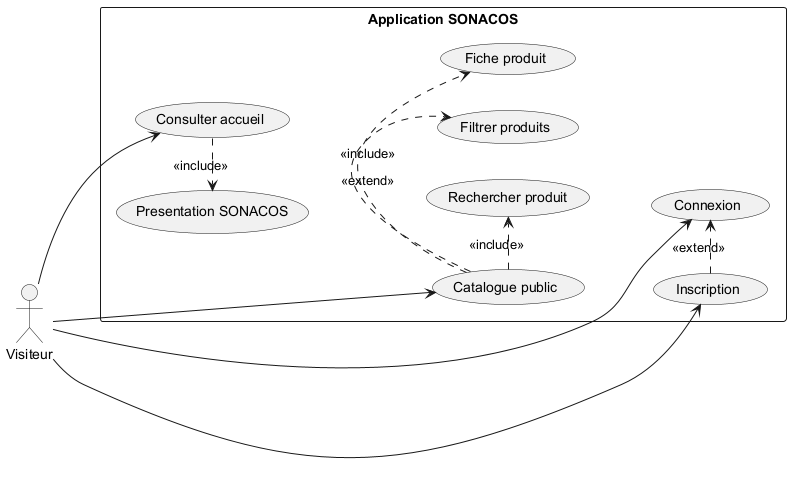
\includegraphics[width=0.92\textwidth,height=0.62\textheight,keepaspectratio]{usecase_visiteur.png}
  \caption{Diagramme PlantUML des cas d'utilisation du visiteur}
  \label{fig:uc-plantuml-visiteur}
\end{figure}

\paragraph{Objectif.}
Le visiteur utilise l'application sans authentification pour decouvrir l'offre SONACOS, consulter les produits disponibles et acceder aux pages d'inscription ou de connexion.

\paragraph{Scenario nominal.}
\begin{enumerate}
  \item Le visiteur ouvre la page d'accueil de l'application.
  \item Le systeme affiche une présentation claire de SONACOS, les grandes familles de produits et les acces principaux.
  \item Le visiteur ouvre le catalogue public.
  \item Le systeme affiche les produits actifs avec image, famille, reference, disponibilite, prix en MAD, conditionnement, stock et livraison.
  \item Le visiteur recherche un produit par nom ou reference.
  \item Le systeme conserve les criteres et affiche les resultats correspondants.
  \item Le visiteur clique sur une carte produit.
  \item Le systeme ouvre la fiche produit complète dans une page dediee.
\end{enumerate}

\paragraph{Cas alternatifs.}
\begin{itemize}
  \item Si aucun produit ne correspond à la recherche, le systeme affiche un etat vide clair.
  \item Si le visiteur veut commander, le systeme l'oriente vers la connexion ou l'inscription.
  \item Si un produit n'est plus actif, il n'apparait plus dans le catalogue public.
\end{itemize}

\subsubsection{Client}

\begin{figure}[H]
  \centering
  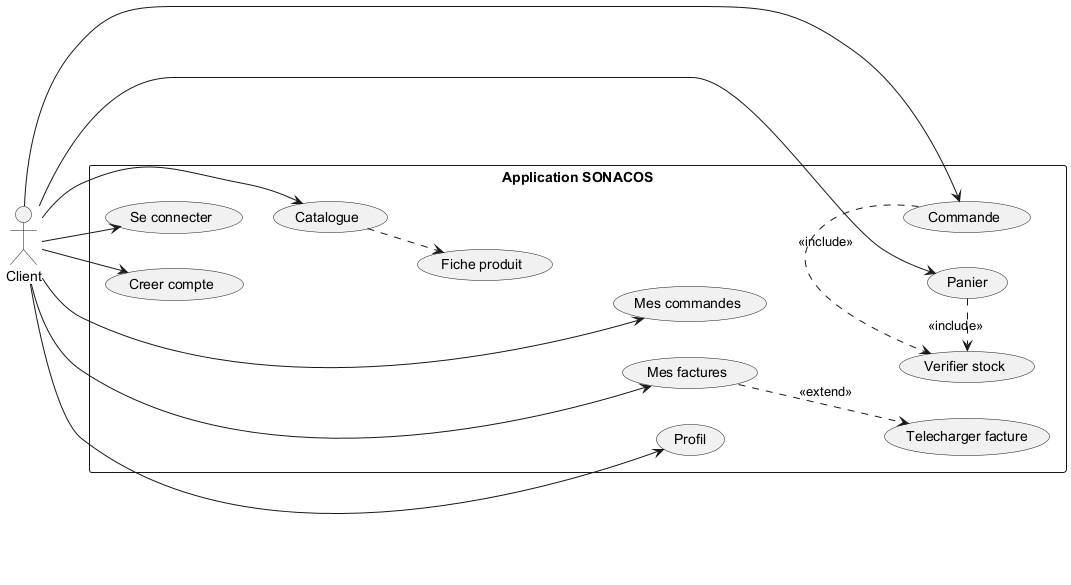
\includegraphics[width=0.92\textwidth,height=0.62\textheight,keepaspectratio]{usecase_client.png}
  \caption{Diagramme PlantUML des cas d'utilisation du client}
  \label{fig:uc-plantuml-client}
\end{figure}

\paragraph{Objectif.}
Le client prepare ses achats depuis le catalogue, gere son panier, passe commande, suit l'avancement et telecharge ses factures lorsque celles-ci sont disponibles.

\paragraph{Preconditions.}
\begin{itemize}
  \item Le client possede un compte actif ou cree un compte depuis la page d'inscription.
  \item Les produits commandes doivent etre actifs et disposer d'un stock suffisant.
  \item Les factures sont telechargeables uniquement apres generation par le systeme.
\end{itemize}

\paragraph{Scenario nominal.}
\begin{enumerate}
  \item Le client se connecte avec son adresse e-mail et son mot de passe.
  \item Le back-end verifie les identifiants et retourne un jeton JWT.
  \item Le front-end redirige le client vers son espace personnel.
  \item Le client consulte le catalogue et ouvre une fiche produit.
  \item Il ajoute un produit au panier en choisissant une quantite.
  \item Le systeme calcule le sous-total de la ligne et le total du panier.
  \item Le client modifie si besoin la quantite ou supprime un article.
  \item Le client confirme la commande.
  \item Le systeme contrôle le stock, cree la commande et enregistre les lignes commandees.
  \item Le client consulte la commande dans son historique.
  \item Lorsque la facture existe, le client la telecharge depuis son espace factures.
\end{enumerate}

\paragraph{Cas alternatifs.}
\begin{itemize}
  \item Si le mot de passe est incorrect, le systeme affiche un message d'erreur sans connecter l'utilisateur.
  \item Si le stock est insuffisant, la commande n'est pas validee et le client est informe.
  \item Si la facture n'est pas encore disponible, le bouton de telechargement reste indisponible ou affiche un message explicite.
  \item Si le compte est desactive par l'administrateur, la connexion est refusee.
\end{itemize}

\subsubsection{Gestionnaire}

\begin{figure}[H]
  \centering
  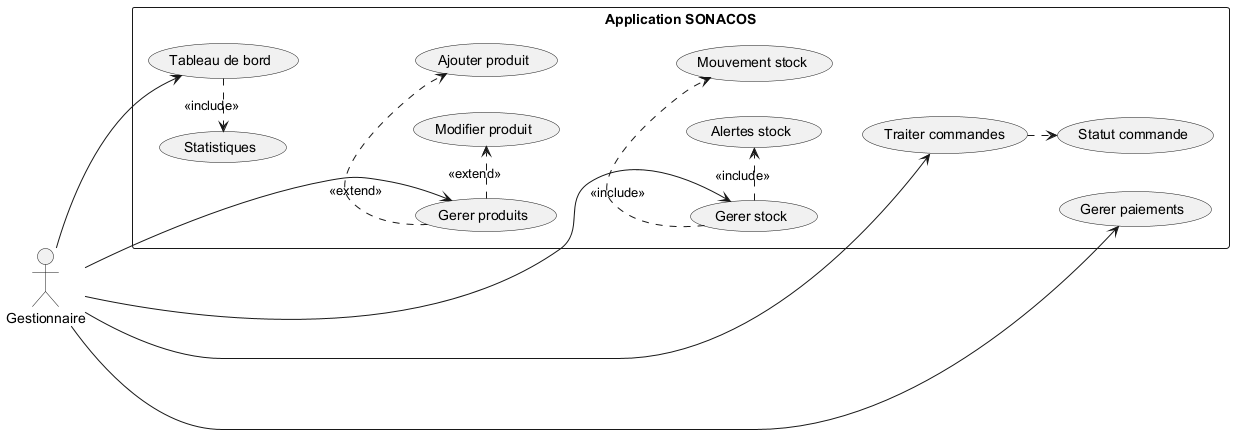
\includegraphics[width=0.92\textwidth,height=0.62\textheight,keepaspectratio]{usecase_gestionnaire.png}
  \caption{Diagramme PlantUML des cas d'utilisation du gestionnaire}
  \label{fig:uc-plantuml-gestionnaire}
\end{figure}

\paragraph{Objectif.}
Le gestionnaire pilote les opérations commerciales et logistiques : produits, stock, commandes, paiements et indicateurs utiles au suivi quotidien.

\paragraph{Preconditions.}
\begin{itemize}
  \item L'utilisateur doit etre authentifie avec le role \texttt{GESTIONNAIRE}.
  \item Les actions d'ajout ou de modification de produit doivent respecter les champs obligatoires : nom, reference, categorie, prix, conditionnement et stock.
  \item Les mouvements de stock doivent etre lies a un produit existant.
\end{itemize}

\paragraph{Scenario nominal de gestion produit.}
\begin{enumerate}
  \item Le gestionnaire ouvre l'espace produits.
  \item Le systeme affiche la liste paginee des produits avec recherche et filtres.
  \item Le gestionnaire ajoute une nouvelle reference ou modifie un produit existant.
  \item Il renseigne le nom, la reference, la categorie, le prix, le conditionnement, la description et l'image.
  \item Le systeme valide les champs et enregistre la modification.
  \item Le produit devient visible ou masque dans le catalogue selon son statut actif.
\end{enumerate}

\paragraph{Scenario nominal de gestion stock.}
\begin{enumerate}
  \item Le gestionnaire ouvre le module stock.
  \item Il choisit un produit et le type de mouvement : entree, sortie ou correction.
  \item Il renseigne la quantite et le motif.
  \item Le systeme met a jour le stock disponible.
  \item Le mouvement est historise pour permettre le contrôle ulterieur.
\end{enumerate}

\paragraph{Cas alternatifs.}
\begin{itemize}
  \item Si la reference produit existe deja, le systeme refuse l'enregistrement.
  \item Si une sortie de stock depasse la quantite disponible, le systeme bloque l'operation.
  \item Si une commande est deja finalisee, certaines modifications deviennent indisponibles.
\end{itemize}

\subsubsection{Responsable}

\begin{figure}[H]
  \centering
  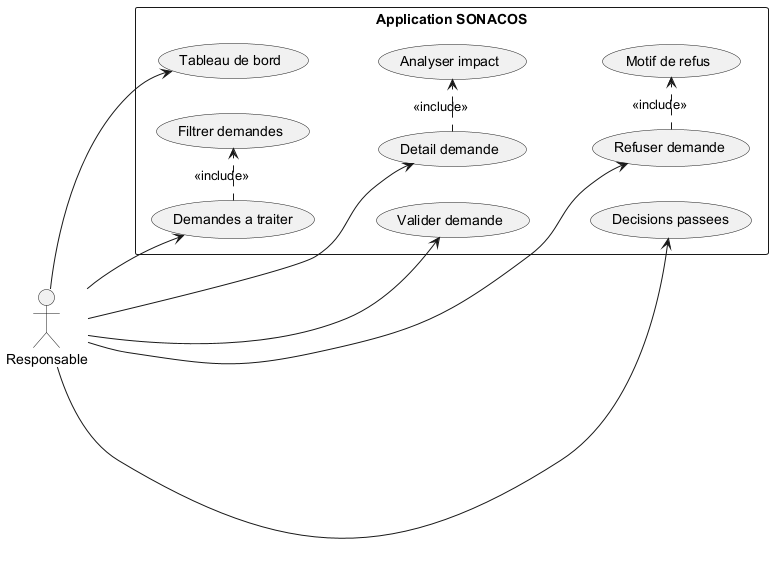
\includegraphics[width=0.92\textwidth,height=0.62\textheight,keepaspectratio]{usecase_responsable.png}
  \caption{Diagramme PlantUML des cas d'utilisation du responsable}
  \label{fig:uc-plantuml-responsable}
\end{figure}

\paragraph{Objectif.}
Le responsable contrôle les opérations necessitant une decision : validations sensibles, refus motives et consultation de l'historique des decisions.

\paragraph{Scenario nominal.}
\begin{enumerate}
  \item Le responsable ouvre son tableau de bord.
  \item Le systeme affiche le nombre de demandes en attente, les urgences et les decisions recentes.
  \item Le responsable filtre les demandes par type, priorite ou statut.
  \item Il ouvre le detail d'une demande.
  \item Le systeme presente l'objet concerne, le demandeur, l'impact commercial ou stock et les informations utiles.
  \item Le responsable valide la demande si elle est conforme.
  \item Le systeme met a jour le statut et trace la decision dans le journal.
\end{enumerate}

\paragraph{Cas de refus.}
\begin{enumerate}
  \item Le responsable clique sur refuser.
  \item Le systeme impose la saisie d'un motif.
  \item Le responsable renseigne le motif de refus.
  \item Le systeme enregistre la decision, le motif, la date et l'utilisateur responsable.
\end{enumerate}

\paragraph{Cas alternatifs.}
\begin{itemize}
  \item Si la demande a deja ete traitee par un autre responsable, elle n'est plus modifiable.
  \item Si le motif de refus est vide, le systeme bloque la decision.
  \item Si une erreur API se produit, le statut local n'est pas modifie.
\end{itemize}

\subsubsection{Administrateur}

\begin{figure}[H]
  \centering
  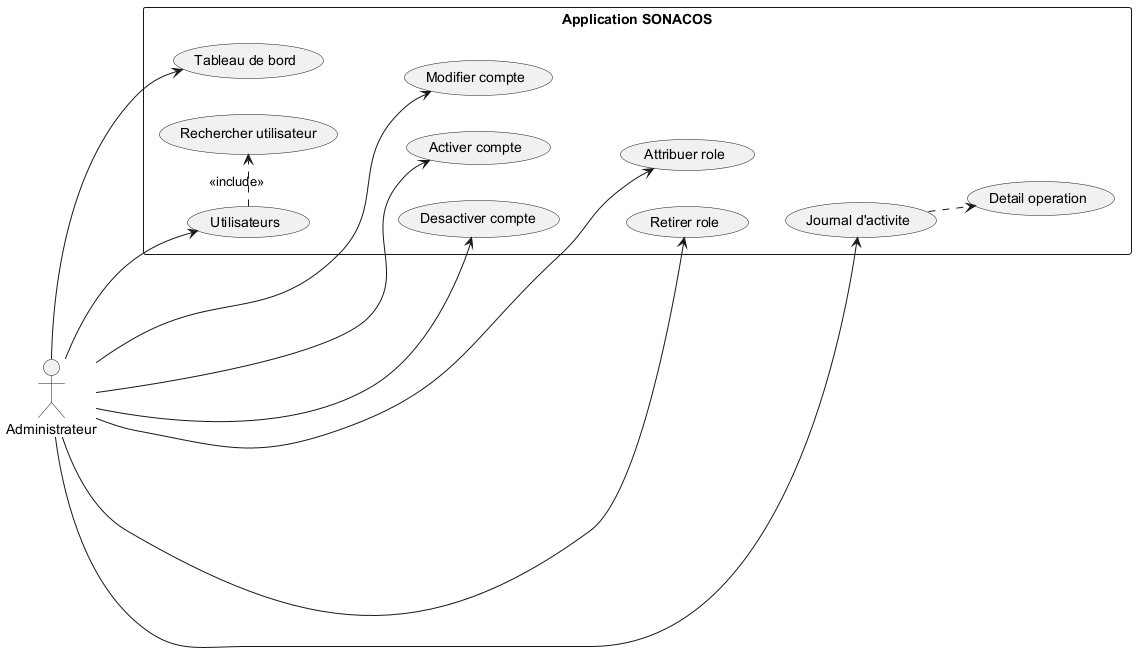
\includegraphics[width=0.92\textwidth,height=0.62\textheight,keepaspectratio]{usecase_admin.png}
  \caption{Diagramme PlantUML des cas d'utilisation de l'administrateur}
  \label{fig:uc-plantuml-admin}
\end{figure}

\paragraph{Objectif.}
L'administrateur gere la securite fonctionnelle de l'application : utilisateurs, activation des comptes, attribution des roles et consultation du journal d'activite.

\paragraph{Preconditions.}
\begin{itemize}
  \item L'utilisateur doit etre authentifie avec le role \texttt{ADMIN}.
  \item Les roles disponibles doivent exister dans le systeme.
  \item Les actions administratives doivent etre tracees.
\end{itemize}

\paragraph{Scenario nominal de modification utilisateur.}
\begin{enumerate}
  \item L'administrateur ouvre la page utilisateurs.
  \item Le systeme affiche la liste des comptes avec nom, email, ville, role, date de creation et statut.
  \item L'administrateur recherche un utilisateur.
  \item Il ouvre l'action modifier.
  \item Le systeme affiche les informations modifiables du compte.
  \item L'administrateur met a jour les champs autorises.
  \item Le systeme sauvegarde et affiche la nouvelle version du compte.
\end{enumerate}

\paragraph{Scenario nominal de gestion des roles.}
\begin{enumerate}
  \item L'administrateur selectionne un utilisateur.
  \item Il ajoute ou retire un role applicatif.
  \item Le systeme verifie que la modification est autorisee.
  \item Le systeme met a jour les droits d'acces.
  \item L'action est ajoutee au journal d'activite.
\end{enumerate}

\paragraph{Cas alternatifs.}
\begin{itemize}
  \item Si l'administrateur tente de retirer son propre role critique, le systeme doit empecher une perte d'acces.
  \item Si un compte est desactive, l'utilisateur concerne ne peut plus se connecter.
  \item Si une operation administrative echoue, le systeme conserve l'ancien etat.
\end{itemize}

\subsubsection{Archiviste}

\begin{figure}[H]
  \centering
  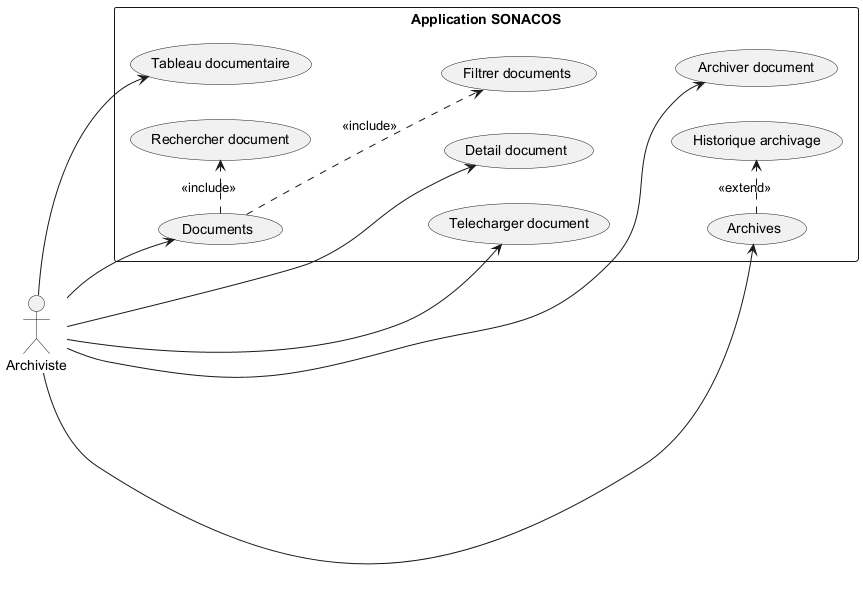
\includegraphics[width=0.92\textwidth,height=0.62\textheight,keepaspectratio]{usecase_archiviste.png}
  \caption{Diagramme PlantUML des cas d'utilisation de l'archiviste}
  \label{fig:uc-plantuml-archiviste}
\end{figure}

\paragraph{Objectif.}
L'archiviste centralise, consulte, telecharge et classe les documents commerciaux, principalement les factures et documents associes aux commandes.

\paragraph{Scenario nominal.}
\begin{enumerate}
  \item L'archiviste ouvre son tableau de bord documentaire.
  \item Le systeme affiche les documents disponibles, archives et en attente.
  \item L'archiviste filtre par type, statut ou date.
  \item Il ouvre le detail d'un document.
  \item Il telecharge le document pour vérification.
  \item Lorsque le document est conforme, il lance l'archivage.
  \item Le systeme marque le document comme archive et conserve l'historique.
\end{enumerate}

\paragraph{Cas alternatifs.}
\begin{itemize}
  \item Si le fichier PDF n'existe pas, le telechargement est bloque avec un message clair.
  \item Si le document est deja archive, le systeme evite un double archivage.
  \item Si l'utilisateur n'a pas le role archiviste, l'acces au module est refuse.
\end{itemize}

\subsubsection{Auditeur}

\begin{figure}[H]
  \centering
  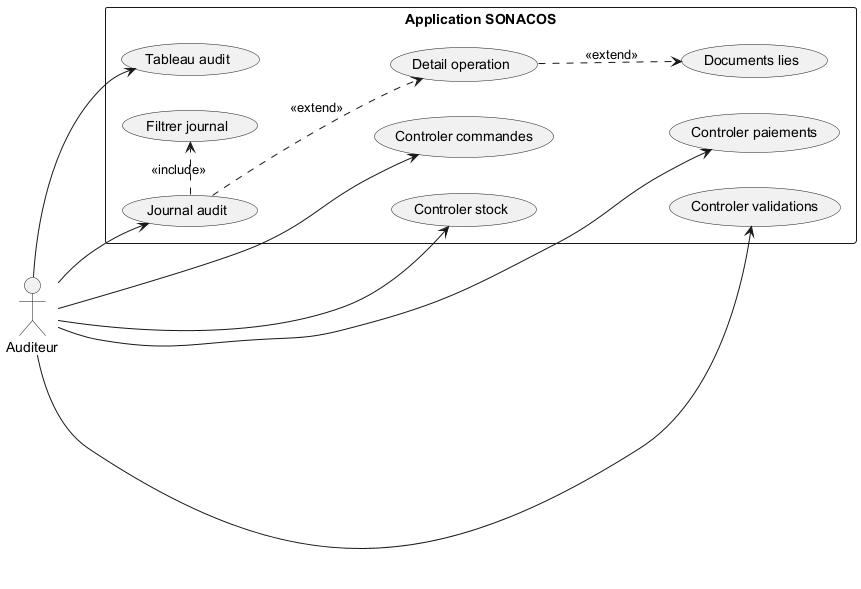
\includegraphics[width=0.92\textwidth,height=0.62\textheight,keepaspectratio]{usecase_auditeur.png}
  \caption{Diagramme PlantUML des cas d'utilisation de l'auditeur}
  \label{fig:uc-plantuml-auditeur}
\end{figure}

\paragraph{Objectif.}
L'auditeur contrôle les opérations sensibles en lecture seule. Il ne modifie pas les données, mais verifie la cohérence des commandes, paiements, stocks, validations et journaux.

\paragraph{Scenario nominal.}
\begin{enumerate}
  \item L'auditeur ouvre le tableau de bord audit.
  \item Le systeme affiche les indicateurs de contrôle et les opérations recentes.
  \item L'auditeur ouvre le journal d'audit.
  \item Il filtre par module, acteur, type d'action ou date.
  \item Il ouvre le detail d'une operation.
  \item Le systeme affiche l'utilisateur, l'action, l'objet concerne, la date et les informations associees.
  \item L'auditeur compare les informations avec les commandes, mouvements de stock, paiements ou validations.
\end{enumerate}

\paragraph{Cas alternatifs.}
\begin{itemize}
  \item Si aucune operation ne correspond aux filtres, un etat vide est affiche.
  \item Si l'operation n'existe plus, le systeme affiche une page d'information au lieu d'une erreur technique.
  \item Si l'auditeur tente une action de modification, le front-end et le back-end doivent la refuser.
\end{itemize}


\section{Diagramme de classes}

Le diagramme de classes represente les entites principales : utilisateur, role, categorie, produit, panier, commande, paiement, facture, mouvement de stock, validation et historique.

\begin{figure}[H]
  \centering
  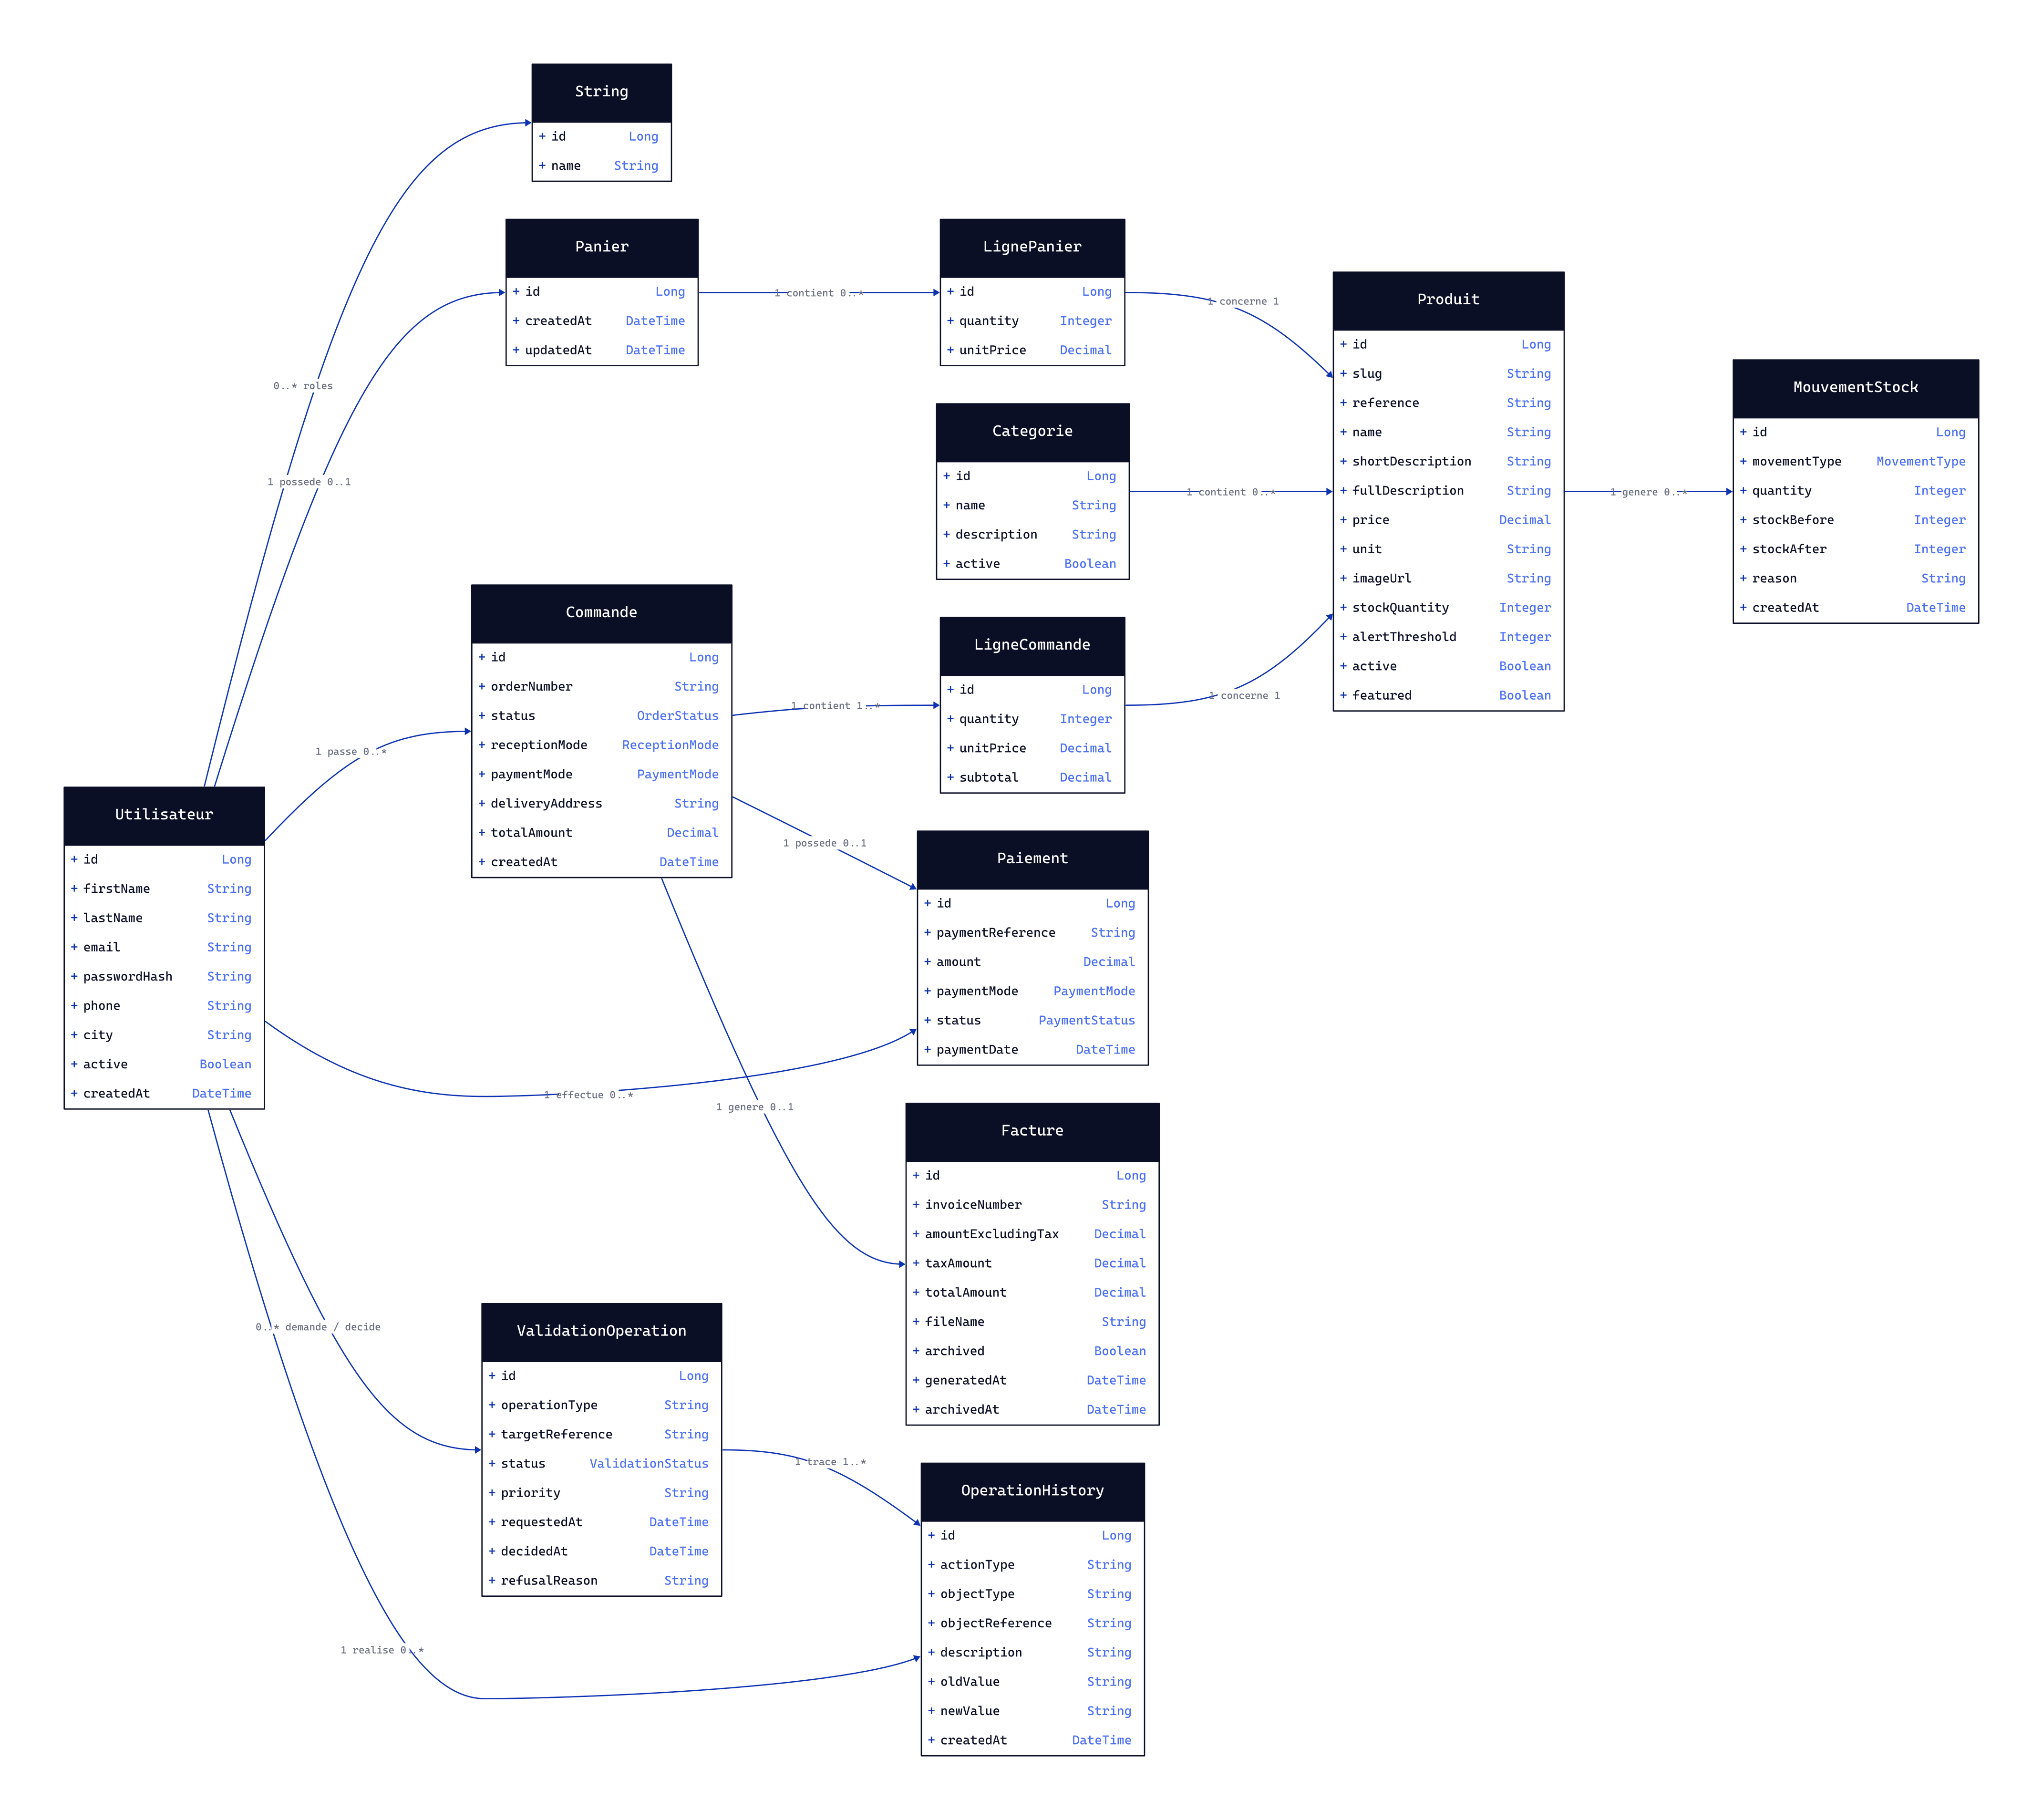
\includegraphics[width=0.95\textwidth,height=0.62\textheight,keepaspectratio]{class_global.png}
  \caption{Diagramme de classes global}
  \label{fig:class-global}
\end{figure}

\section{Diagrammes de sequence}

\subsection{Commande, paiement et facture}

Ce diagramme de sequence montre le parcours principal d'un client : connexion, consultation du catalogue, ajout au panier, confirmation de commande, vérification du stock, paiement et generation de facture.

\begin{figure}[H]
  \centering
  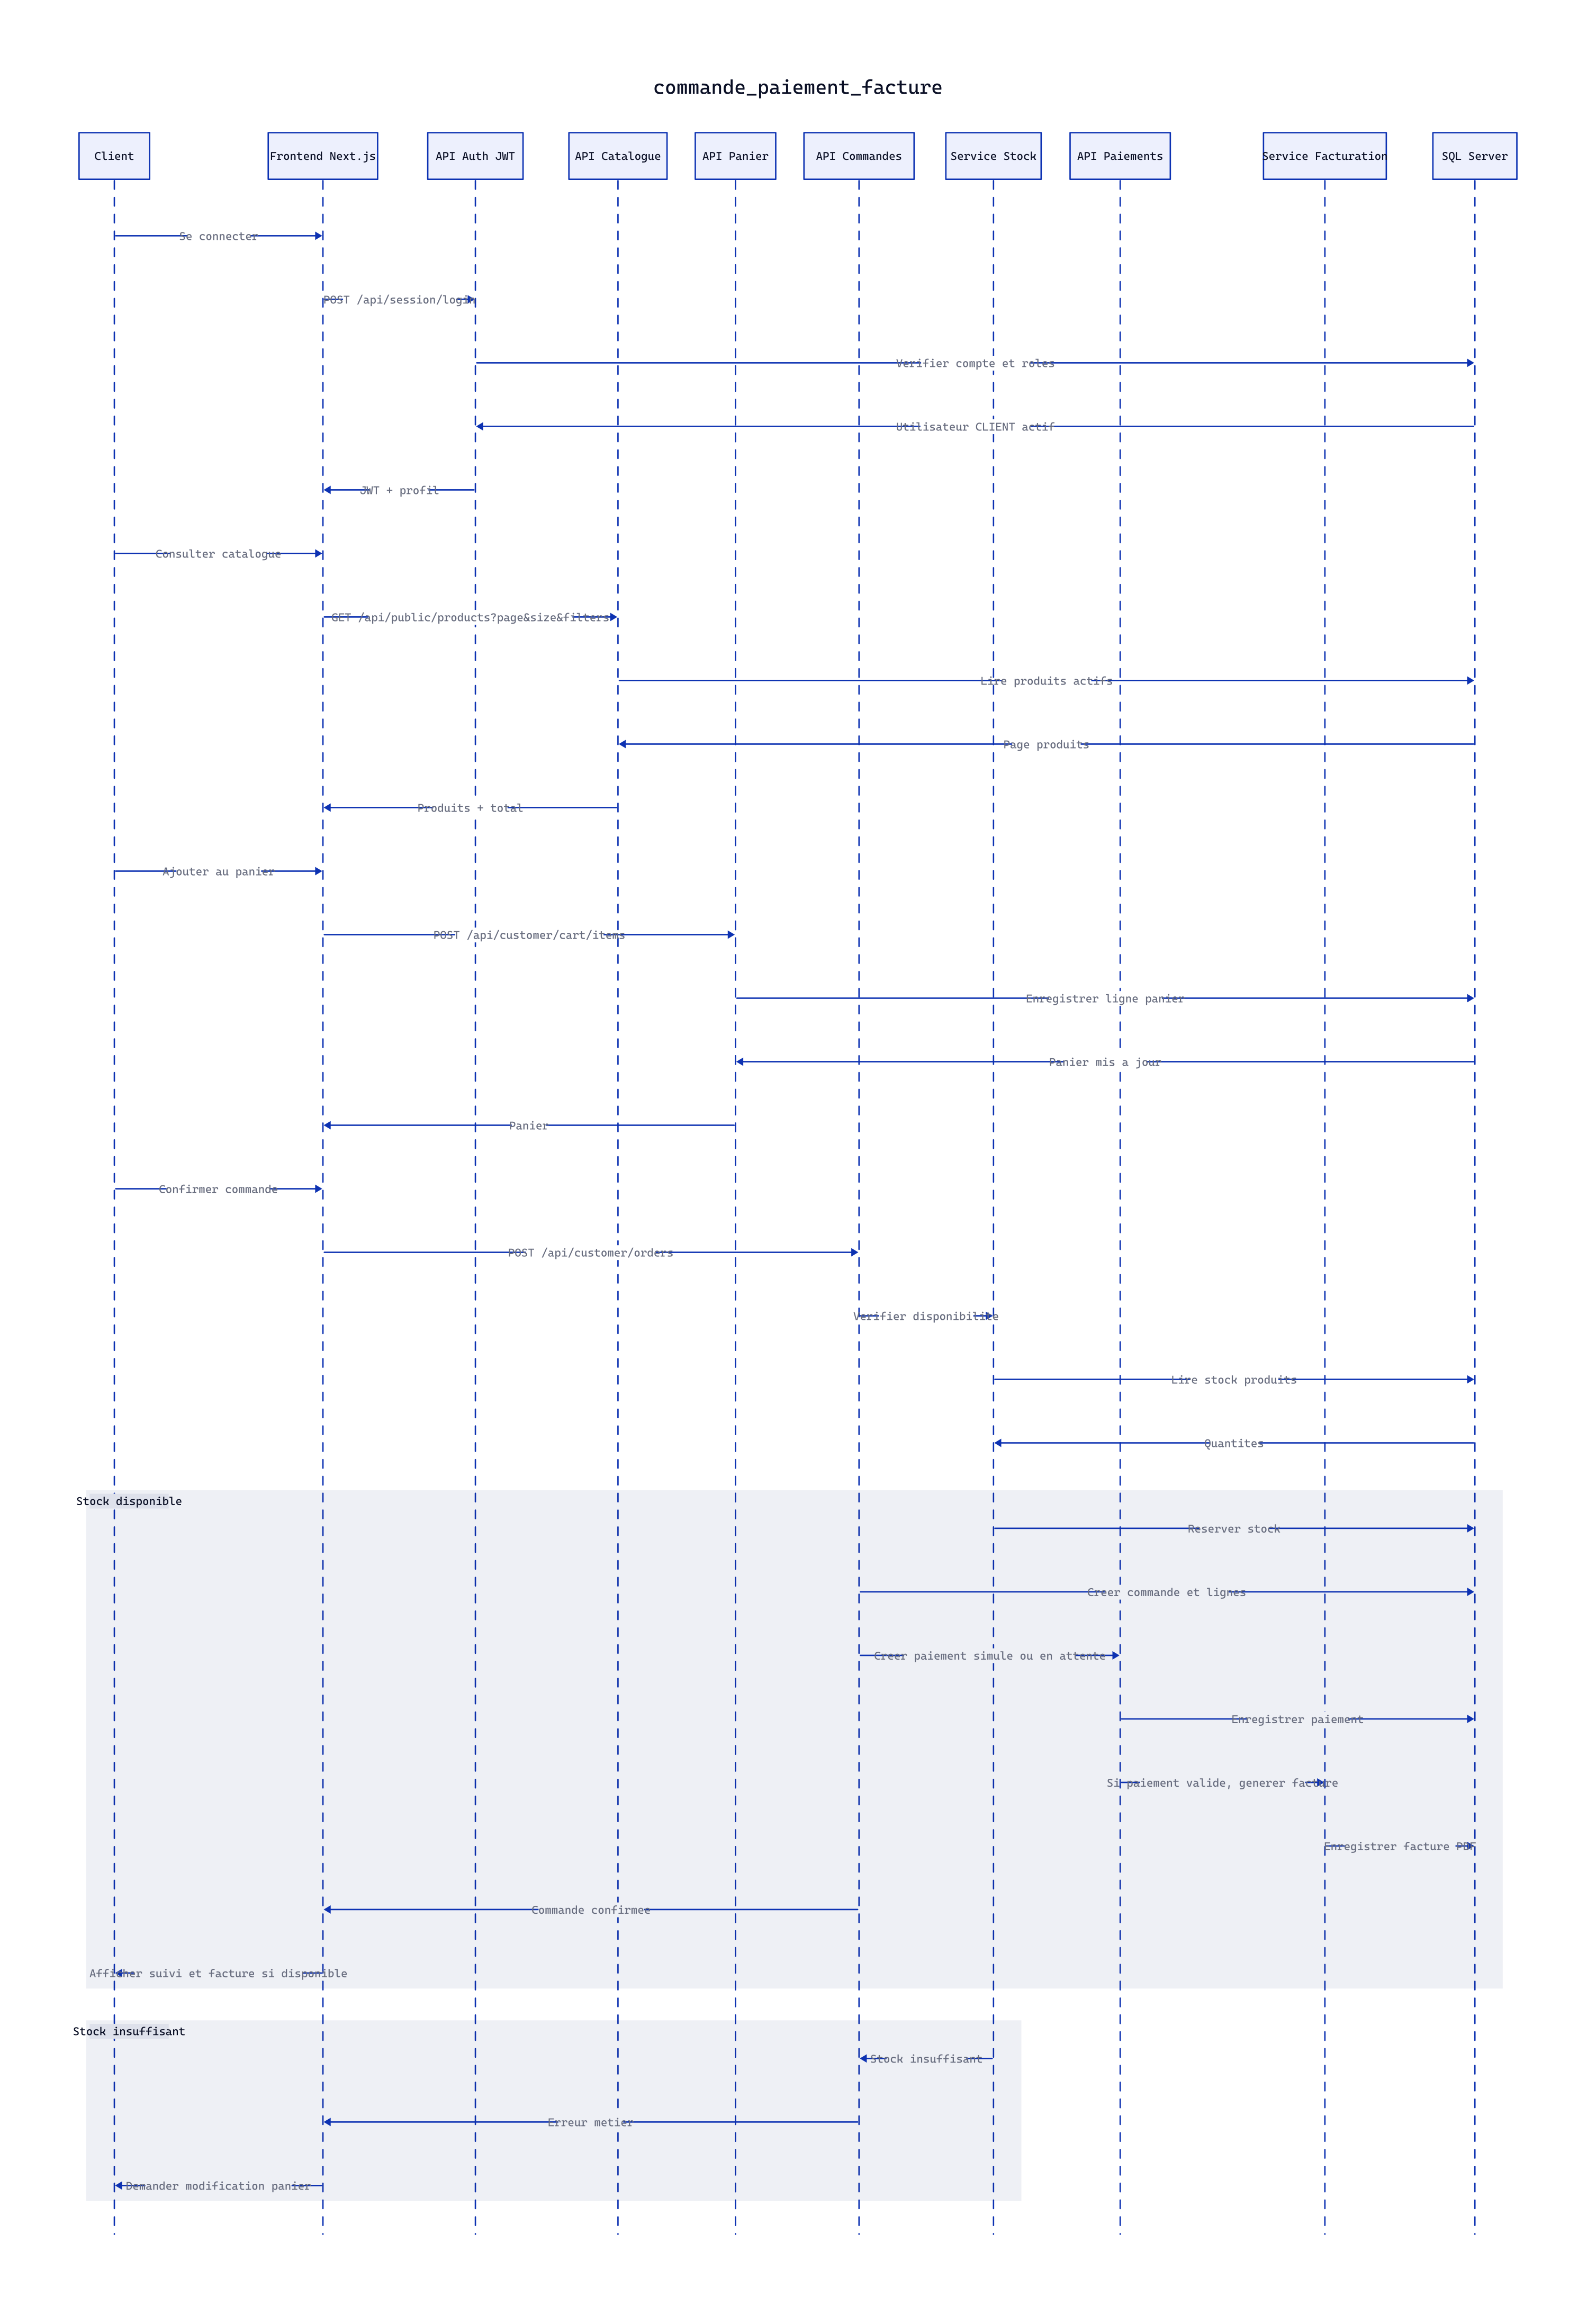
\includegraphics[width=0.95\textwidth,height=0.62\textheight,keepaspectratio]{sequence_commande_paiement_facture.png}
  \caption{Diagramme de sequence : commande, paiement et facture}
  \label{fig:sequence-commande}
\end{figure}

\subsection{Administration des utilisateurs}

L'administrateur peut consulter les comptes, modifier les informations, activer ou desactiver un utilisateur et attribuer des roles. Chaque action sensible est tracee dans le journal.

\begin{figure}[H]
  \centering
  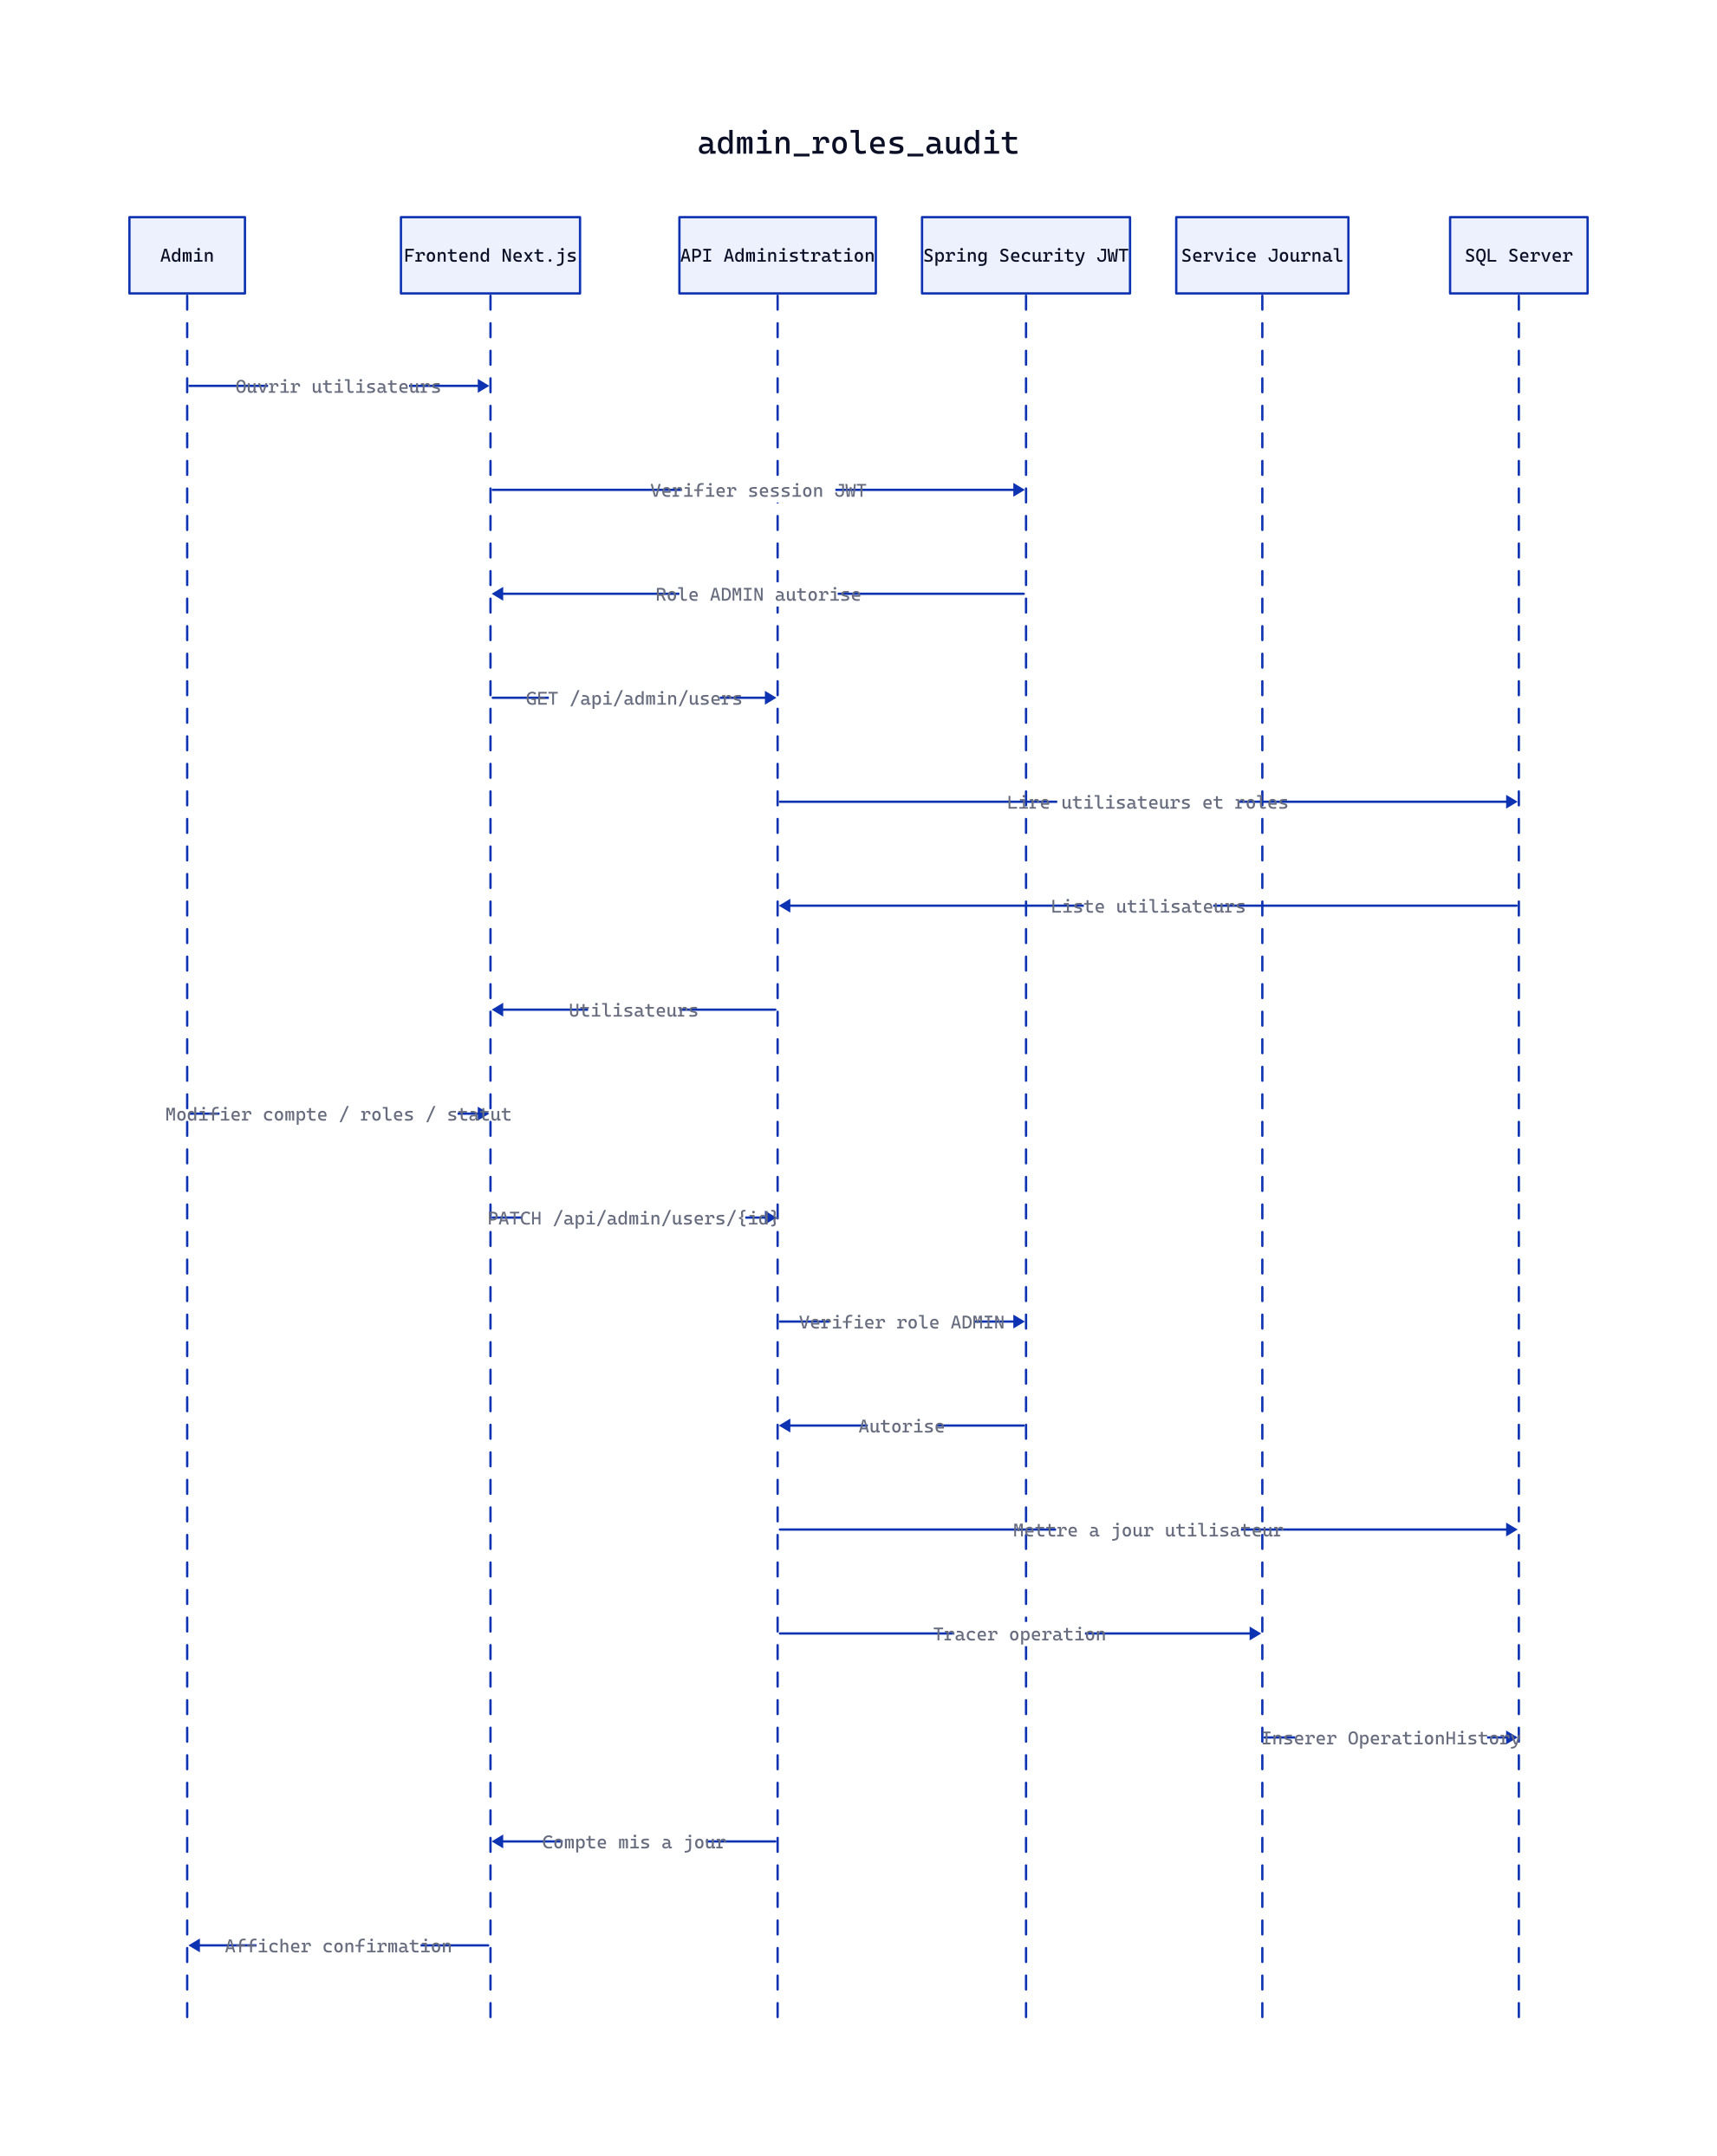
\includegraphics[width=0.95\textwidth,height=0.68\textheight,keepaspectratio]{sequence_admin_roles_audit.png}
  \caption{Diagramme de sequence : administration des utilisateurs}
  \label{fig:sequence-admin}
\end{figure}

\subsection{Archivage et audit}

L'archiviste gere l'archivage documentaire tandis que l'auditeur consulte les journaux en lecture seule. Cette separation renforce la tracabilite des opérations.

\begin{figure}[H]
  \centering
  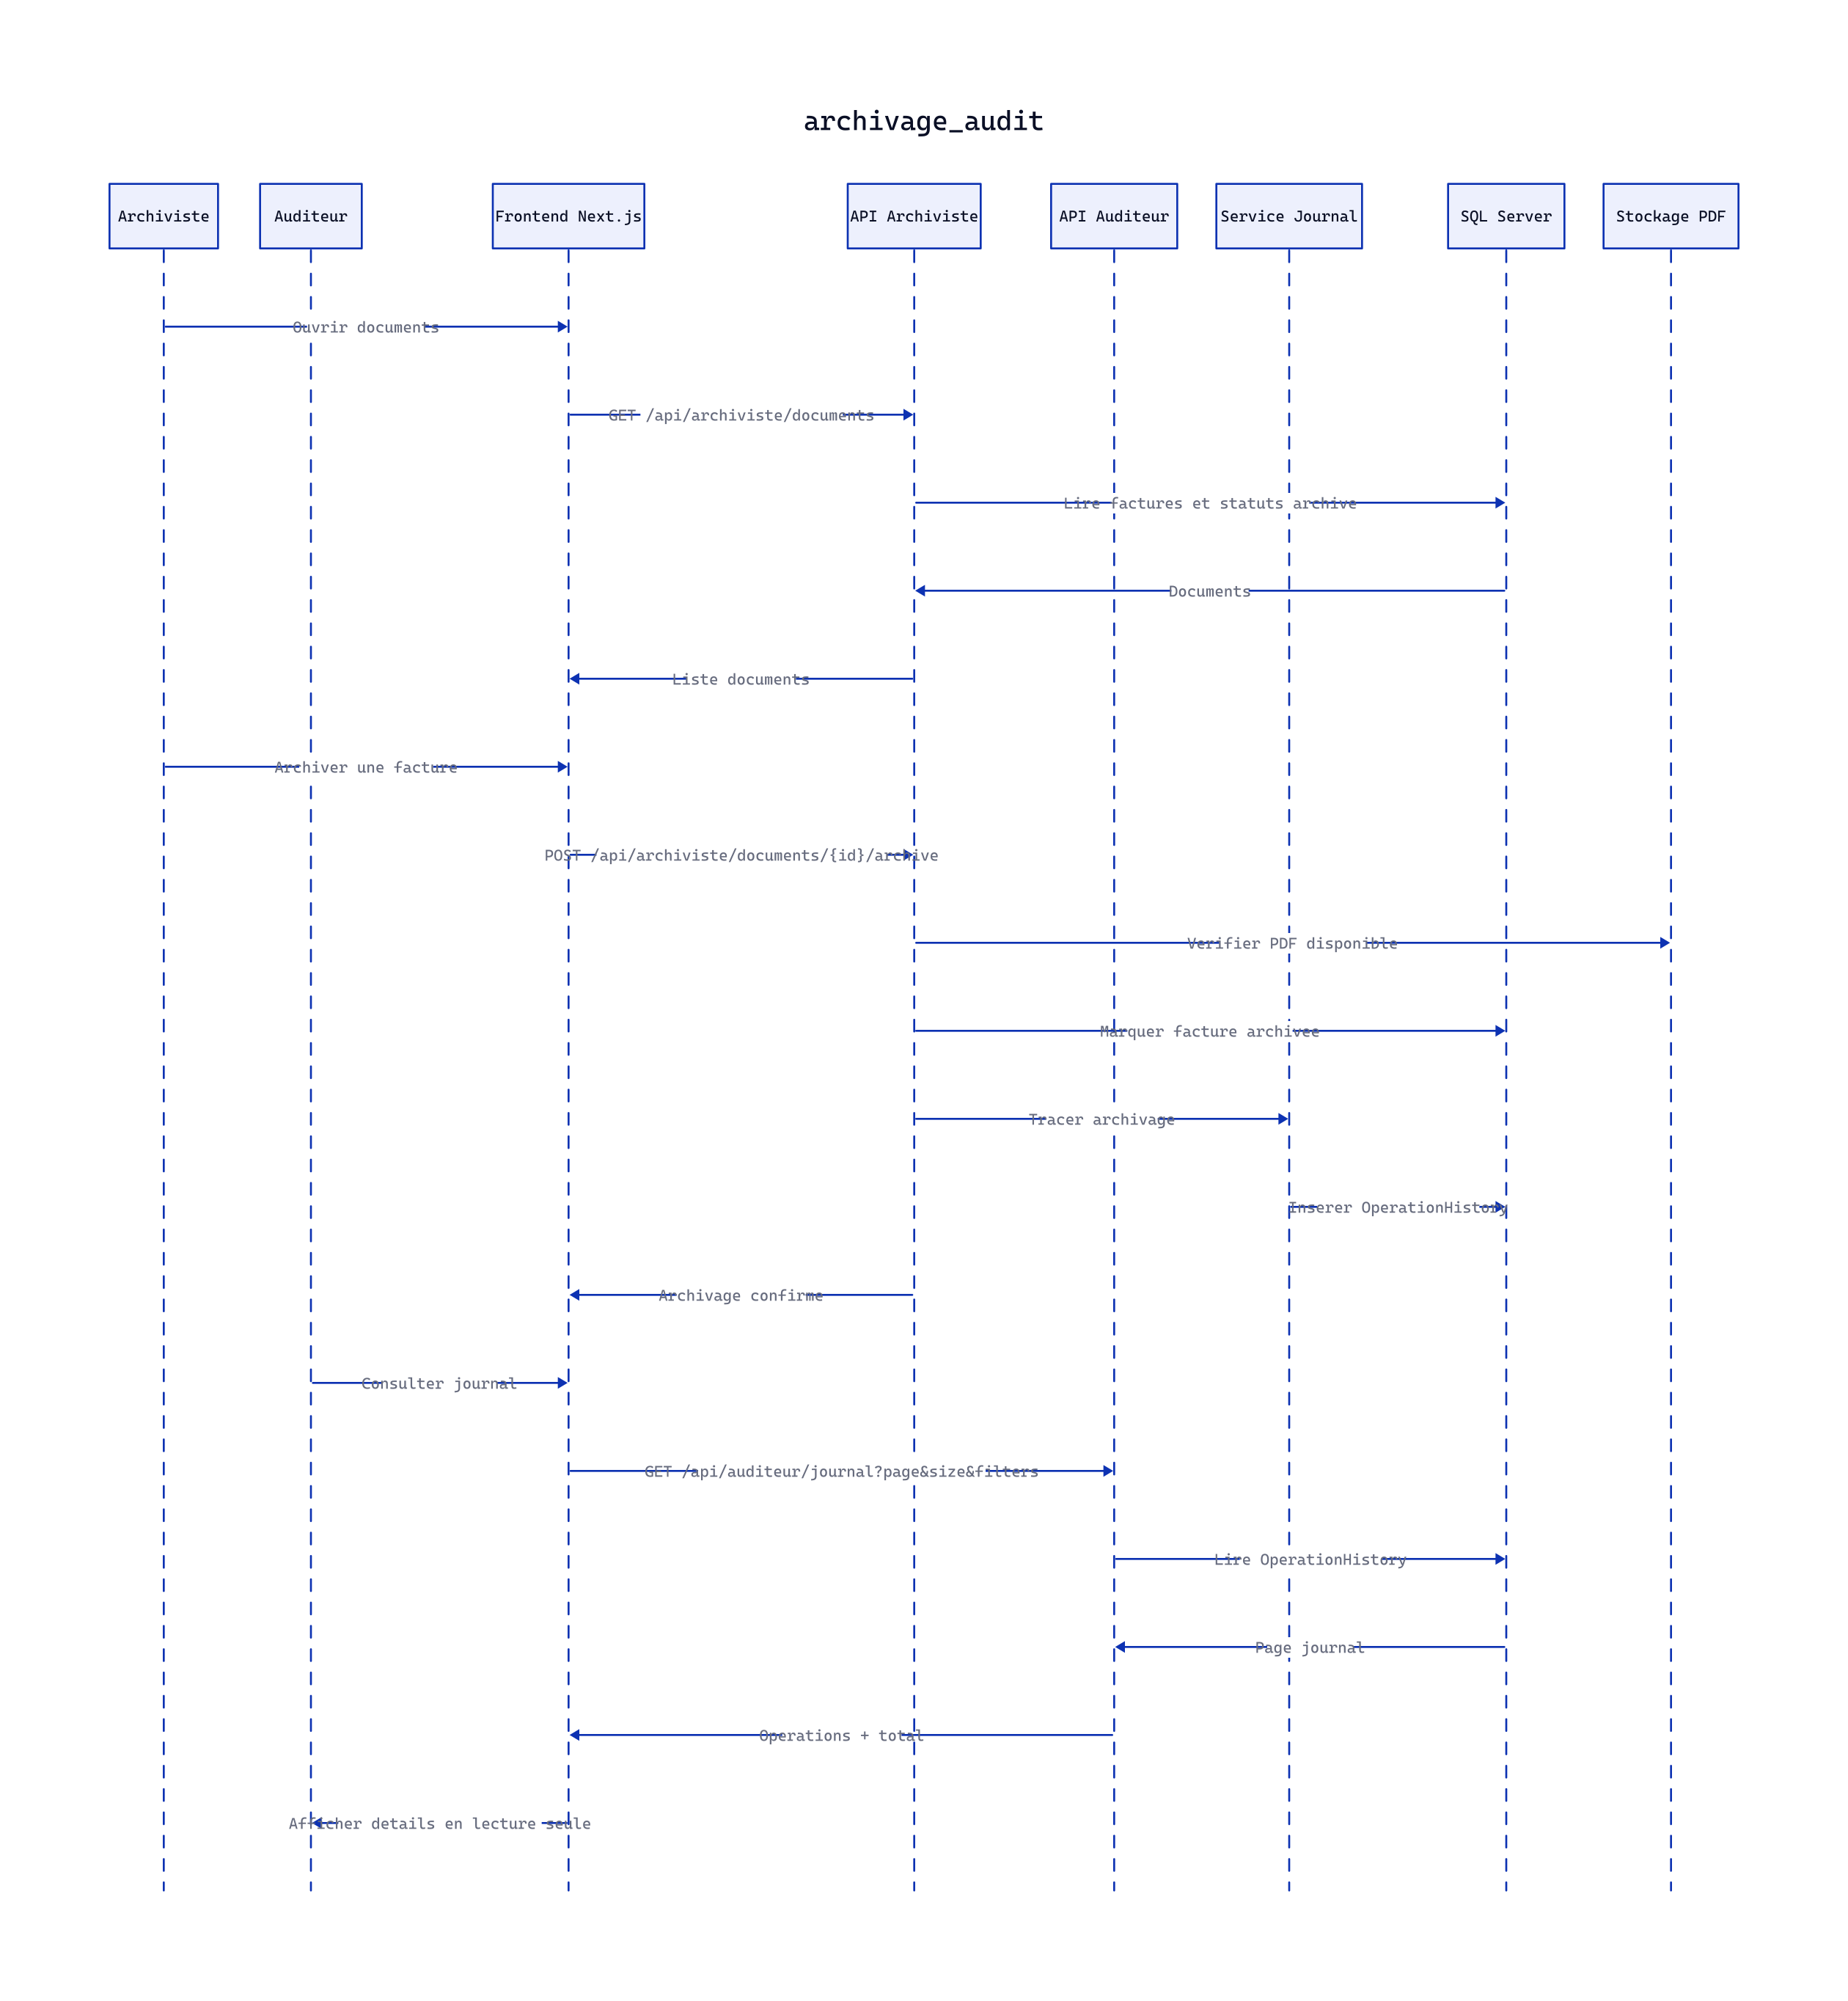
\includegraphics[width=0.95\textwidth,height=0.68\textheight,keepaspectratio]{sequence_archivage_audit.png}
  \caption{Diagramme de sequence : archivage et audit}
  \label{fig:sequence-archivage}
\end{figure}

\section{Diagramme d'activite}

Le diagramme d'activite represente le traitement global d'une commande, depuis la consultation du catalogue jusqu'a l'archivage et l'audit.

\begin{figure}[H]
  \centering
  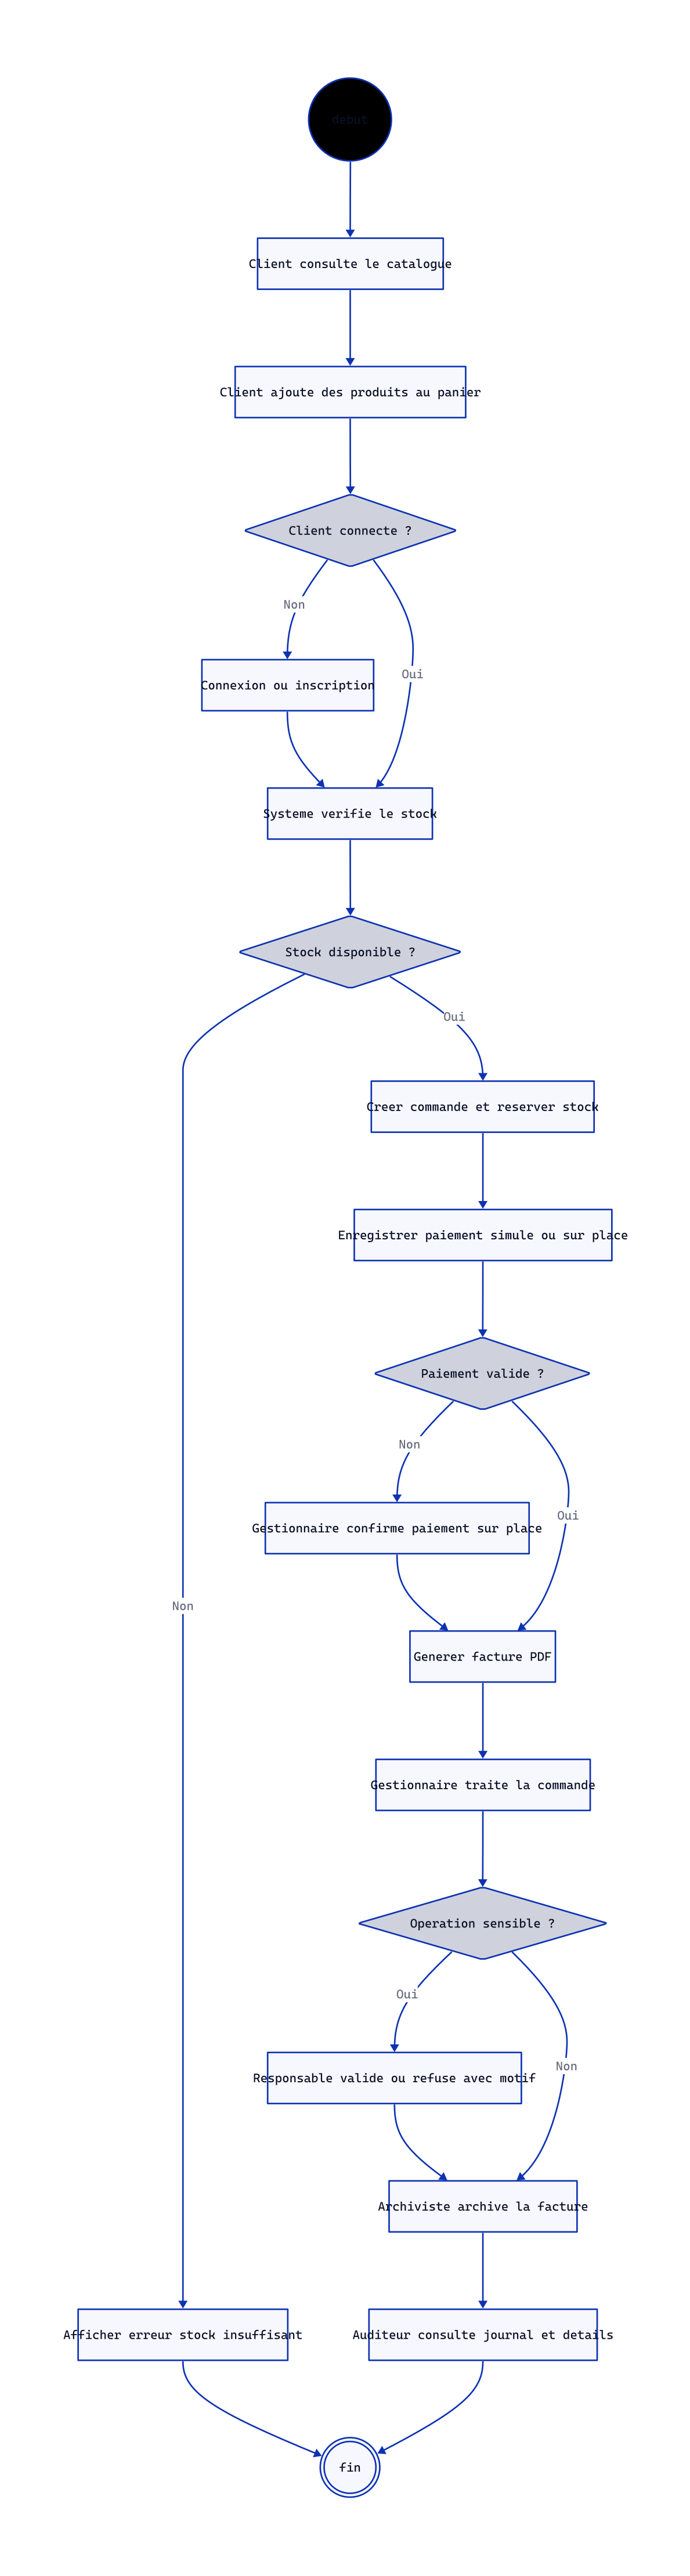
\includegraphics[width=0.95\textwidth,height=0.72\textheight,keepaspectratio]{activity_traitement_commande_global.png}
  \caption{Diagramme d'activite : traitement global d'une commande}
  \label{fig:activity-commande}
\end{figure}

\chapter{Réalisation et mise en oeuvre}

\section{Architecture generale}

L'application suit une architecture web en trois couches :

\begin{itemize}
  \item la couche présentation, developpee avec Next.js et React ;
  \item la couche metier, developpee avec Spring Boot ;
  \item la couche données, basee sur SQL Server.
\end{itemize}

\begin{table}[H]
\centering
\caption{Architecture technique du projet}
\begin{tabular}{|p{4cm}|p{10cm}|}
\hline
\textbf{Couche} & \textbf{Technologies et role} \\
\hline
Front-end & Next.js, React, TypeScript, interfaces responsives, espaces utilisateurs. \\
\hline
Back-end & Spring Boot, API REST, services metier, securite JWT. \\
\hline
Base de données & SQL Server, stockage des utilisateurs, produits, commandes, paiements, factures et historiques. \\
\hline
Documentation API & Swagger / OpenAPI pour presenter et tester les endpoints. \\
\hline
\end{tabular}
\end{table}

\section{Technologies utilisées}

\subsection{Front-end}

Le front-end est developpe avec Next.js, React et TypeScript. Il contient les pages publiques, les espaces par role, les composants reutilisables, les formulaires, les tableaux, les cartes produits, les filtres et la pagination.

\subsection{Back-end}

Le back-end est developpe avec Spring Boot. Il expose des API REST permettant la gestion des produits, des commandes, du panier, des paiements, des factures, des validations, des utilisateurs et des journaux d'activite.

\subsection{Base de données}

La base de données utilisée est SQL Server. Elle stocke les données principales de l'application : utilisateurs, roles, categories, produits, commandes, paiements, factures, mouvements de stock et historiques.

\subsection{Securite}

La securite repose sur Spring Security et JWT. Apres connexion, l'utilisateur recoit une session permettant d'acceder uniquement aux ressources autorisees. Les roles definissent les droits d'acces.

\section{Structure fonctionnelle de l'application}

\begin{longtable}{|p{4cm}|p{10cm}|}
\caption{Espaces fonctionnels de la plateforme}\\
\hline
\textbf{Espace} & \textbf{Fonctionnalites principales} \\
\hline
\endfirsthead
\hline
\textbf{Espace} & \textbf{Fonctionnalites principales} \\
\hline
\endhead
Public & Accueil, catalogue, recherche, filtres, fiches produits, connexion et inscription. \\
\hline
Client & Tableau de bord, panier, commandes, factures, profil. \\
\hline
Gestionnaire & Produits, stock, mouvements, commandes, paiements, statistiques. \\
\hline
Responsable & Demandes en attente, decisions, validation, refus avec motif. \\
\hline
Administrateur & Utilisateurs, roles, activation/desactivation, journal d'activite. \\
\hline
Archiviste & Documents, factures, archives, telechargements. \\
\hline
Auditeur & Journal d'audit, commandes, stock, paiements, factures et validations en lecture seule. \\
\hline
\end{longtable}

\section{Interfaces de l'application}

\subsection{Accueil}

La page d'accueil presente la plateforme SONACOS, son orientation agricole et les principaux acces de navigation.

\desktopfigure{01-accueil-desktop.png}{Interface d'accueil}{fig:accueil}

\subsection{Catalogue public}

Le catalogue public permet la consultation des produits sans authentification. Les prix sont affiches en MAD et les produits sont organises par categorie.

\desktopfigure{02-catalogue-desktop.png}{Catalogue public}{fig:catalogue}

La grille du catalogue met en avant les produits reels de demonstration avec leur famille, leur image, leur reference, leur disponibilite, leur prix en MAD, le conditionnement, le stock restant et le mode de livraison.

\begin{figure}[H]
  \centering
  \fbox{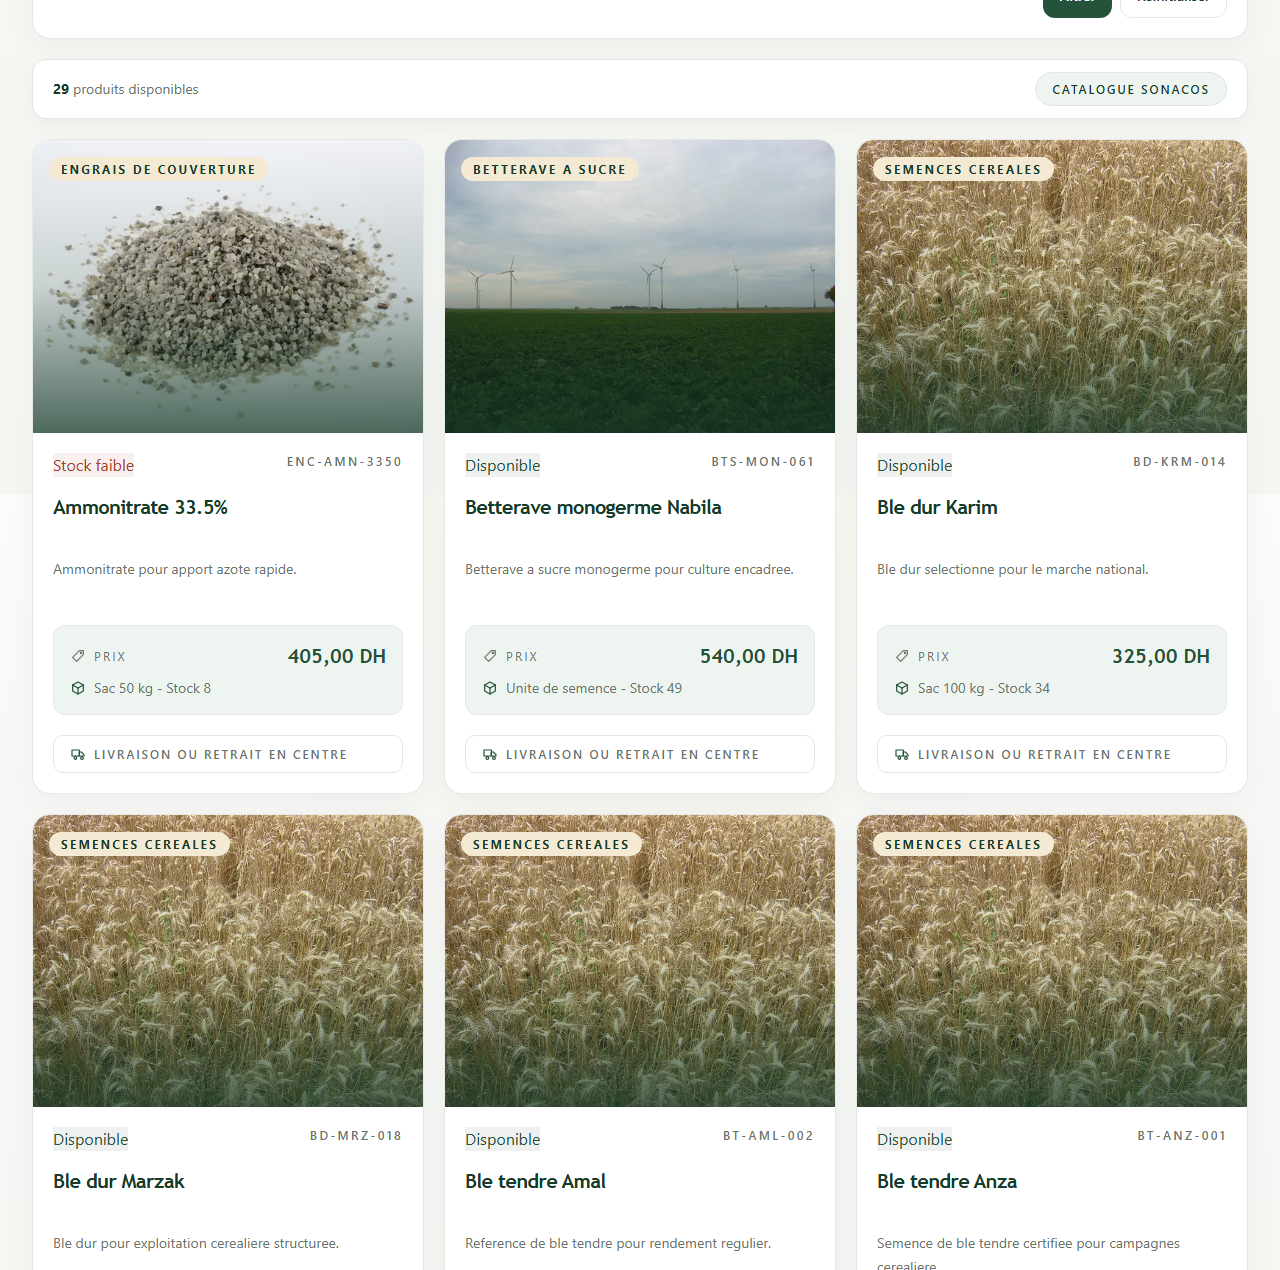
\includegraphics[width=0.86\textwidth,height=0.55\textheight,keepaspectratio]{13-catalogue-produits-grille.png}}
  \caption{Vue détaillee de la grille des produits du catalogue}
  \label{fig:catalogue-produits}
\end{figure}

\begin{figure}[H]
  \centering
  \fbox{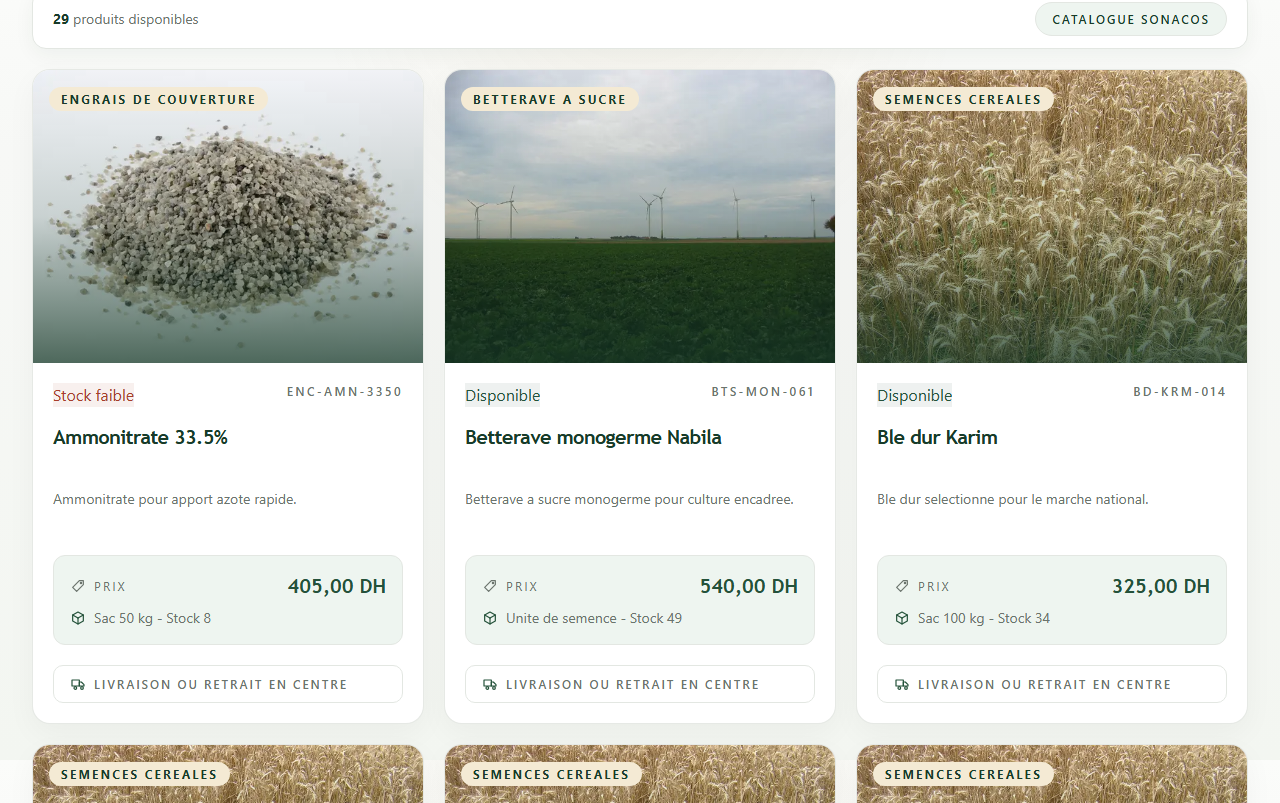
\includegraphics[width=0.9\textwidth,height=0.48\textheight,keepaspectratio]{14-cartes-produits-detail.png}}
  \caption{Cartes produits avec disponibilite, reference, prix, stock et livraison}
  \label{fig:cartes-produits}
\end{figure}

\subsection{Connexion}

La page de connexion permet aux utilisateurs d'acceder a leur espace selon leur role.

\desktopfigure{03-connexion-desktop.png}{Page de connexion}{fig:connexion}

\subsection{Espace client}

L'espace client permet de consulter les commandes, les factures, le panier et le profil.

\desktopfigure{04-client-dashboard-desktop.png}{Tableau de bord client}{fig:client-dashboard}

\desktopfigure{05-client-panier-desktop.png}{Panier client}{fig:client-panier}

\subsection{Espace gestionnaire}

L'espace gestionnaire regroupe les opérations commerciales et logistiques : produits, stock, commandes et paiements.

\desktopfigure{06-gestionnaire-dashboard-desktop.png}{Tableau de bord gestionnaire}{fig:gestionnaire-dashboard}

\desktopfigure{07-gestionnaire-produits-desktop.png}{Gestion des produits}{fig:gestion-produits}

\subsection{Espace responsable}

Le responsable consulte les opérations a traiter et prend les decisions de validation ou de refus.

\desktopfigure{08-responsable-validations-desktop.png}{Gestion des validations}{fig:validations}

\subsection{Espace administrateur}

L'administrateur gere les utilisateurs, les roles et consulte le journal d'activite.

\desktopfigure{09-admin-utilisateurs-desktop.png}{Gestion des utilisateurs}{fig:admin-utilisateurs}

\desktopfigure{10-admin-activite-desktop.png}{Journal d'activite administrateur}{fig:admin-activite}

\subsection{Espace archiviste}

L'archiviste consulte les factures, les documents et les archives disponibles.

\desktopfigure{11-archiviste-documents-desktop.png}{Gestion des documents}{fig:archiviste-documents}

\subsection{Espace auditeur}

L'auditeur dispose d'une consultation en lecture seule des journaux et des activites sensibles.

\desktopfigure{12-auditeur-journal-desktop.png}{Journal d'audit}{fig:auditeur-journal}

\section{Securite et gestion des roles}

L'application repose sur une logique de contrôle d'acces. Chaque role dispose de droits limites :

\begin{itemize}
  \item le visiteur accede uniquement aux pages publiques ;
  \item le client accede a ses propres commandes et factures ;
  \item le gestionnaire agit sur les produits, le stock, les commandes et les paiements ;
  \item le responsable valide ou refuse les opérations ;
  \item l'administrateur gere les comptes et les roles ;
  \item l'archiviste gere les documents ;
  \item l'auditeur consulte les opérations en lecture seule.
\end{itemize}

\section{Pagination, recherche et ergonomie}

Les tableaux et listes importantes disposent d'une recherche, de filtres et d'une pagination numerotee. L'utilisateur peut choisir le nombre d'elements par page : 10, 20, 50 ou 100. Le choix est synchronise avec l'URL afin de conserver l'etat de navigation.

\section{Tests et vérification}

Les vérifications réalisées pendant le développement comprennent :

\begin{itemize}
  \item vérification TypeScript du front-end ;
  \item vérification ESLint ;
  \item build de production Next.js ;
  \item tests Gradle du back-end ;
  \item vérification manuelle des roles et des principales navigations ;
  \item vérification des telechargements de factures disponibles.
\end{itemize}

\chapter{Bilan et perspectives}

\section{Bilan du travail réalisé}

Le projet a permis de concevoir et réalisér une application web complète couvrant les besoins principaux d'une plateforme commerciale SONACOS. La solution offre une consultation publique du catalogue, un espace client fonctionnel, des espaces internes par role et une tracabilite des opérations sensibles.

La réalisation a egalement permis de mettre en pratique plusieurs compétences : analyse des besoins, modélisation UML, conception de base de données, développement front-end, développement back-end, sécurisation par JWT et integration d'interfaces responsives.

\section{Difficultes rencontrees}

Les principales difficultés concernaient :

\begin{itemize}
  \item la separation claire des responsabilites entre les roles ;
  \item la cohérence entre les maquettes, les données et les fonctionnalites reelles ;
  \item la mise en place de listes paginees, filtrees et consultables sur plusieurs espaces ;
  \item la préparation d'une application suffisamment complète pour une demonstration académique.
\end{itemize}

\section{Perspectives d'amélioration}

Plusieurs améliorations peuvent etre envisagees :

\begin{itemize}
  \item integration d'une passerelle de paiement reelle ;
  \item ajout de notifications par e-mail ou SMS ;
  \item gestion avancee des centres regionaux ;
  \item suivi logistique des livraisons ;
  \item generation de rapports statistiques avances ;
  \item archivage documentaire plus complet ;
  \item deploiement en environnement cloud.
\end{itemize}

\chapter*{Conclusion generale}
\addcontentsline{toc}{chapter}{Conclusion generale}

Ce projet de fin d'année avait pour objectif la conception et la réalisation d'une plateforme web de gestion commerciale et e-commerce pour SONACOS. L'application developpee repond aux besoins principaux identifies : consultation du catalogue, gestion du panier, commandes, stock, paiements, factures, validations, administration, archivage et audit.

La solution proposee reste volontairement simple et realiste pour un PFA, tout en étant suffisamment complète pour demontrer une maîtrise des technologies utilisées. L'utilisation de Next.js, Spring Boot, SQL Server et JWT permet d'obtenir une architecture claire, maintenable et sécurisée.

En conclusion, ce projet represente une experience importante de mise en pratique des compétences techniques et methodologiques acquises durant la formation. Il constitue egalement une base evolutive pouvant etre enrichie par des fonctionnalites avancees dans une version future.

\chapter*{References}
\addcontentsline{toc}{chapter}{References}

\section*{Webographie}

\begin{enumerate}
  \item OpenJS Foundation, \textit{Documentation officielle Node.js}. [En ligne]. Disponible : \url{https://nodejs.org/docs/}. Consulte le : 02 septembre 2026.
  \item Vercel, \textit{Documentation officielle Next.js}. [En ligne]. Disponible : \url{https://nextjs.org/docs}. Consulte le : 02 septembre 2026.
  \item Meta Open Source, \textit{Documentation officielle React}. [En ligne]. Disponible : \url{https://react.dev/}. Consulte le : 02 septembre 2026.
  \item Spring, \textit{Documentation officielle Spring Boot}. [En ligne]. Disponible : \url{https://spring.io/projects/spring-boot}. Consulte le : 02 septembre 2026.
  \item Microsoft, \textit{Documentation Microsoft SQL Server}. [En ligne]. Disponible : \url{https://learn.microsoft.com/sql/sql-server/}. Consulte le : 02 septembre 2026.
  \item Auth0, \textit{Introduction aux JSON Web Tokens}. [En ligne]. Disponible : \url{https://jwt.io/introduction}. Consulte le : 02 septembre 2026.
  \item Object Management Group, \textit{Unified Modeling Language Specification}. [En ligne]. Disponible : \url{https://www.omg.org/spec/UML/}. Consulte le : 02 septembre 2026.
  \item EMSI, \textit{Ecole Marocaine des Sciences de l'Ingenieur}. [En ligne]. Disponible : \url{https://emsi.ma/}. Consulte le : 02 septembre 2026.
  \item Honoris United Universities, \textit{The 1st Pan-African private higher education network}. [En ligne]. Disponible : \url{https://honoris.net/}. Consulte le : 02 septembre 2026.
  \item SONACOS, documents internes et supports institutionnels fournis dans le cadre du projet.
\end{enumerate}

\end{document}
